\huge\documentclass{article}


\usepackage[french]{babel}
\usepackage[utf8]{inputenc}

\usepackage[a4paper,top=2cm,bottom=2cm,left=3cm,right=3cm,marginparwidth=1.75cm]{geometry}


\usepackage{amsmath}
\usepackage{graphicx}
\usepackage[colorlinks=true, allcolors=blue]{hyperref}
\usepackage{caption}
\usepackage{listings}

\setcounter{tocdepth}{5}
\setcounter{secnumdepth}{5}

\title{\textbf{Mémoire du projet PDP Chess}}
\author{Rossignon Morgan, Daniel Karl, Salomode Florian, Beites Marvin, Zucchelli Thomas}

\begin{document}

\maketitle
\centerline{
\includegraphics[scale = 0.5]{img/Universite Bordeaux RVB-02.jpg}}

\huge \centerline{\textbf{PDP CHESS}}

\medskip
Projet de développement d'un moteur de jeu d'échec optimisé, ainsi que de joueurs d'échecs artificiels personnalisables.
\normalsize
\newpage

\tableofcontents
\newpage

\section{Contexte}

\subsection{Introduction au projet}

L'objectif de ce projet est de programmer un joueur d'échecs complet.
\newline
Pour cela, nous avons mis en oeuvre différents algorithmes d'exploration d'arbres classiques ainsi que des fonctions d'évaluations propres au jeu d'échecs. Nous avons développé également un moteur de jeu stable que nous avons essayé d'optimiser au maximum.
\newline
Enfin, l'interface de notre application est réalisée en mode texte car l'aspect graphique n'est pas ce que nous souhaitions étudier.

\subsection{Règles du jeu}

Les échecs sont un jeu de plateau opposant deux joueurs. Parfois considéré comme un sport à part entière et disposant même de ses propres compétitions nationales et internationales, il est de nos jours l'un des jeux les plus reconnus et les plus populaires.

Le plateau où se déroule une partie d'échecs, couramment appelé échiquier, est divisé en soixante-quatre cases qui se divise en cases blanches et noires en damier. 
\begin{figure}[!h]
    \centering
    \includegraphics[scale = 0.35]{img/echiquier.png}
    \caption{Exemple d'échiquier en configuration classique de démarrage d'une partie, \href{https://lichess.org/editor}{lichess.org}}
    \label{fig:echiquier}
\end{figure}


Sur un échiquier, chaque case est couramment associée à la combinaison d'un chiffre et d'une lettre. Elles peuvent aller de A1 correspondant à la case située en bas à gauche, jusqu'à H8 qui est la case située en haut à droite.

Les huit lignes de cases verticales sont nommées colonnes. Chacune des cases composant une colonne possédera la même lettre dans son appellation. Les huit lignes de cases horizontales sont nommées rangées. Chacune des cases composant une rangée possédera le même chiffre dans son appellation.

Au lancement d'une partie, les pièces blanches sont situées sur les rangées numérotées 1 et 2 tandis que les pièces noires se trouvent sur les rangées numérotées 7 et 8.

\subsubsection{Les pièces}

Chaque joueur dispose d'un total de seize pièces, blanches ou noires. Elles sont réparties en huit catégories différentes selon leur façon de se déplacer à travers l'échiquier.

Chaque pièce ne peut se trouver que sur une seule case à la fois. De même, chaque case ne peut accueillir qu'une seule pièce.

\begin{itemize}
    \item Huit pions.
    \item Deux tours.
    \item Deux fous.
    \item Deux cavaliers.
    \item Une reine.
    \item Un roi.
\end{itemize}

Les pièces peuvent alors se diviser en deux catégories. Glissantes et non-glissantes.

\paragraph{Les pièces glissantes}
~~\\

Les pièces glissantes sont celles capables de traverser le plateau en un seul coup. Parmi ces pièces on retrouve :

\begin{itemize}
    \item La tour, capable de se déplacer en haut, bas, gauche et droite.
    \item Le fou, capable de se déplacer en diagonale.
    \item La reine, capable de cumuler les mouvements de la tour et du fou.
\end{itemize}

\begin{figure}[h]
\centering
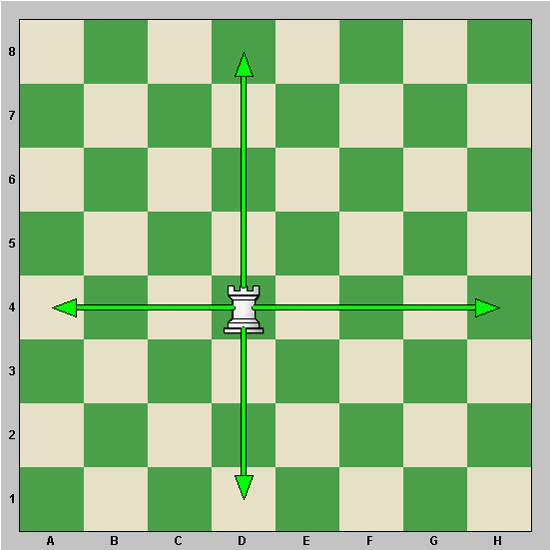
\includegraphics[scale=0.5]{img/mouvements_tour.jpg}
\caption{La tour,
\href{https://www.europe-echecs.com/art/2-le-deplacement-des-pieces-93.html}{europe-echecs.com}}
\end{figure}

\begin{figure}[h]
\centering
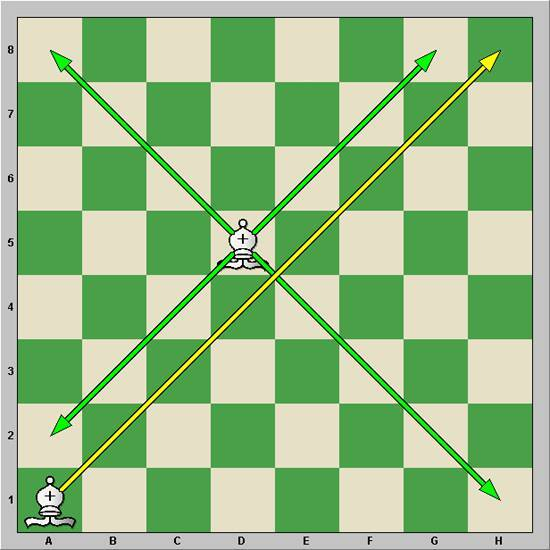
\includegraphics[scale=0.5]{img/mouvements_fou.jpg}
\caption{Le fou,
\href{https://www.europe-echecs.com/art/2-le-deplacement-des-pieces-93.html}{europe-echecs.com}}
\end{figure}

\newpage

\begin{figure}[h]
\centering
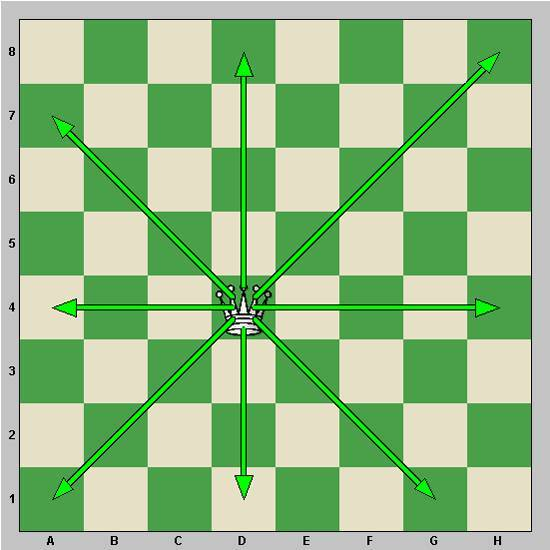
\includegraphics[scale=0.5]{img/mouvements_reine.jpg}
\caption{La reine,
\href{https://www.europe-echecs.com/art/2-le-deplacement-des-pieces-93.html}{europe-echecs.com}}
\end{figure}

\paragraph{Les pièces non-glissantes}
~~\\
Les pièces non-glissantes, à l'inverse des glissantes, ne peuvent se déplacer que d'une seule case, si aucune pièce de la même couleur ne se trouve à la destination (cas particulier pour le pion). Parmi ces pièces on retrouve :

\begin{itemize}
    \item Le pion, capable de se déplacer d'une ou deux cases vers l'avant.
    \item Le roi, capable de se déplacer d'une case dans toutes les directions.
    \item Le cavalier, un peu particulier, capable de se déplacer de deux cases verticalement ou horizontalement puis d'une autre case horizontalement ou verticalement. On ramène souvent cette particularité à un "déplacement en L". De plus, le cavalier est capable de sauter par dessus les autres pièces, tant qu'aucune pièce alliée ne se trouve sur la case à laquelle il doit arriver.
\end{itemize}

\begin{figure}[h]
\centering
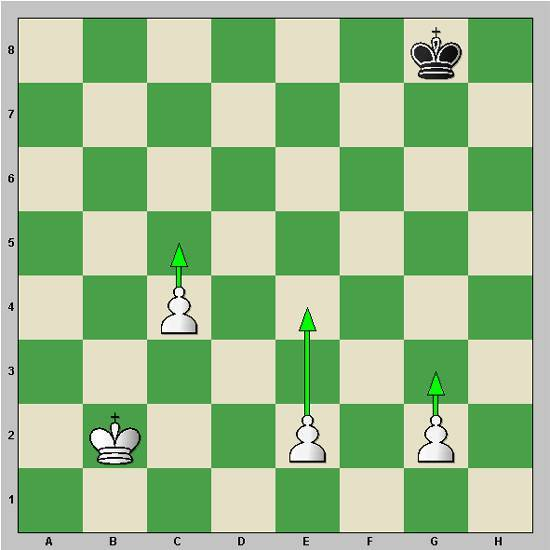
\includegraphics[scale=0.5]{img/mouvements_pion.jpg}
\caption{Le pion,
\href{https://www.europe-echecs.com/art/2-le-deplacement-des-pieces-93.html}{europe-echecs.com}}
\end{figure}

\newpage

\begin{figure}[h]
\centering
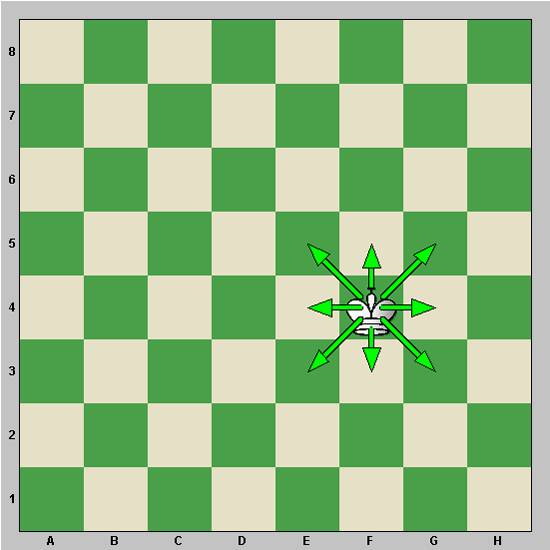
\includegraphics[scale=0.5]{img/mouvements_roi.jpg}
\caption{Le roi,
\href{https://www.europe-echecs.com/art/2-le-deplacement-des-pieces-93.html}{europe-echecs.com}}
\end{figure}

\begin{figure}[h]
\centering
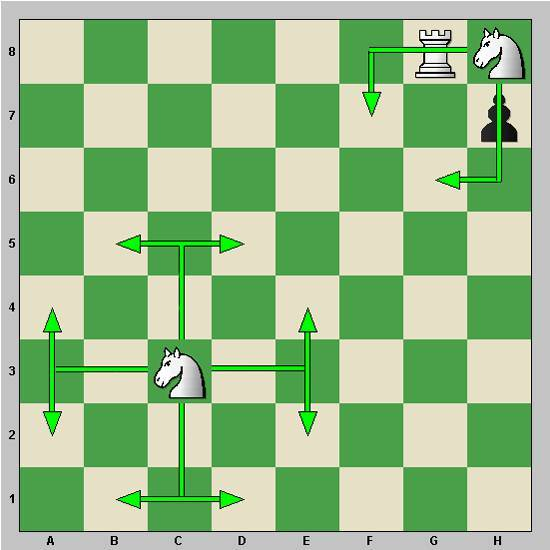
\includegraphics[scale=0.5]{img/mouvements_cavalier.jpg}
\caption{Le cavalier,
\href{https://www.europe-echecs.com/art/2-le-deplacement-des-pieces-93.html}{europe-echecs.com}}
\end{figure}


\subsubsection{Les conditions d'arrêt}\label{condition d'arret}

Aux échecs, il n'y a que deux issues possibles : la victoire de l'un des deux joueurs ou l'égalité. Il existe de multiples situations qui peuvent mener à l'une ou à l'autre.

\paragraph{La victoire}
~~\\

Plusieurs situations peuvent amener à la victoire de l'un des deux joueurs :
\newline

\begin{itemize}
    \item Si l'un des deux joueurs se retrouve dans une position d'échecs et mat. Cette situation se produit si le roi du joueur sera vaincu peu importe le mouvement légal effectué.
    \item Si l'un des deux joueurs décide d'abandonner la partie.
    \item Si l'un des deux joueurs perd au temps. Cette situation se produit uniquement dans le cas d'une partie où chaque joueur dispose d'un temps limité pour effectuer chaque action.
\end{itemize}

L'image ci-dessous présente un exemple d'échecs et mats. En effet, la tour blanche est en position d'éliminer le roi noir qui ne pourra pas y échapper avec une seule action.\newline

\begin{figure}[!h]
\centering
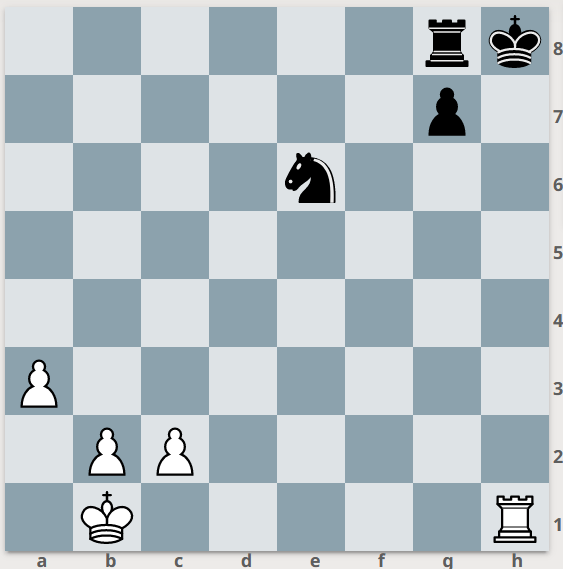
\includegraphics[scale=0.5]{img/echec-et-mat.png}
\caption{L'échec et mat,
\href{https://www.apprendre-les-echecs-24h.com/blog/echec-et-mat/}{apprendre-les-echecs-24h.com}}
\end{figure}

\paragraph{Les matchs nuls}
~~\\

De même, plusieurs situations peuvent amener à un match nul, signifiant qu'aucun des deux joueurs ne pourra obtenir une victoire :

\begin{itemize}
    \item Si les deux joueurs se mettent d'accord au cours de la partie.
    \item Si un plateau de jeu est répété trois fois dans la partie.
    \item Si jamais cinquante coups ont été effectués depuis la dernière capture d'une pièce ou la dernière poussée d'un pion.
    \item Si jamais les deux joueurs se retrouvent dans l'impossibilité de placer leur adversaire dans une position d'échecs et mat.
    \item Si jamais l'un des deux joueurs se retrouve dans l'incapacité d'effectuer un mouvement légal. Si ce cas est généralement considéré comme un match nul, il est de temps en temps considéré comme une défaite pour le joueur incapable de déplacer ses pièces. Cela s'appelle le pat.
\end{itemize}

\begin{figure}[h]
\centering
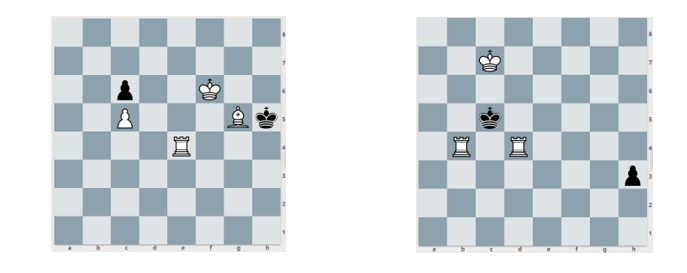
\includegraphics[scale=1]{img/pat.png}
\caption{Le pat,  \href{https://www.apprendre-les-echecs-24h.com/blog/debuter-aux-echecs/le-pat/}{ apprendre-les-echecs-24h.com}}
\end{figure}

L'image ci-dessus permet de démontrer le principe du pat.

Sur l'image de gauche, nous pouvons constater que les pièces noires n'ont pas de coups légaux à leurs disposition. Le pion noir ne peut pas avancer et le roi est également bloqué car un déplacement le mettrait en position d'échec, ce qui est interdit. Dans cette configuration actuelle, le roi n'est pas attaqué. Il s'agît là du pat. Même si les blancs disposent de la supériorité numérique, ce match est nul.

Sur l'image de droite, même si le roi noir ne peut pas se déplacer sans se mettre en échec, il est toujours possible de bouger le pion. Dans ce cas-là, il n'y a pas de pat et la partie continue comme si de rien n'était.

\subsubsection{Les coups spéciaux}

En plus des différents mouvements légaux, il existe également ce qui est appelé communément des coups spéciaux, qui ne se produisent que sous certaines conditions.

\paragraph{La promotion}\label{Promotion}
~~\\

La promotion se produit lorsque l'un des deux joueurs parvient à amener un pion jusqu'à la dernière rangée, soit la rangée numérotée 8 pour les pièces blanches et la 1 pour les pièces noires.

Il est alors possible pour le joueur de transformer ce pion en n'importe quelle autre pièce de son choix, à l'exception du roi. Généralement, la dame est le choix le plus courant. Ce choix se fait indépendamment des pièces déjà présentes sur l'échiquier. Il est donc possible pour un joueur de disposer de deux dames.

\paragraph{Le roque}
~~\\

Le roque est un mouvement spécial impliquant le roi et l'une des tours de l'un des joueurs. Il s'agît de la seule action des échecs permettant le déplacement de deux pièces à la fois sans même respecter les mouvements légaux de ces deux pièces en question.

Le roque ne peut être effectué que dans la situation où le roi et l'une des tours d'un joueur sont encore placées à leur position initiale.

Si aucune pièce ne se trouve entre le roi et la tour alors le joueur peut déplacer le roi de deux cases en direction de la tour et placer ensuite cette même tour juste à côté du roi, de l'autre côté. Une erreur commune est de bouger la tour avant le roi, ce qui est considéré comme un coup illégal. Déplacer le roi en premier est donc primordial.

Il existe deux types de roques : le petit roque et le grand roque. La différence réside dans le nombre de cases que devra effectuer la tour pour se placer à côté du roi. Deux cases dans le cas du petit roque et trois cases dans le cas du grand.

L'image ci-dessous montre les étapes du petit roque blanc et du grand roque noir.

\begin{figure}[h]
\centering
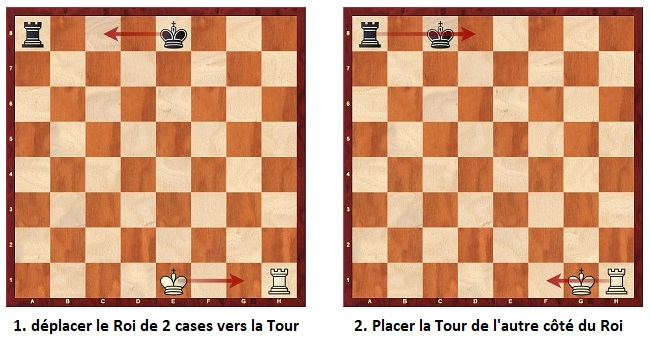
\includegraphics[scale=0.8]{img/roque.jpg}
\caption{Le roque,
\href{https://ecole.apprendre-les-echecs.com/roque/}{ecole.apprendre-les-echecs.com}}
\end{figure}

\paragraph{Le en-passant}
~~\\

Le en-passant est un mouvement spécial qui concerne les pions.

Dans la situation où un pion se trouve sur la cinquième rangée, si un pion adverse dans sa position initiale effectue un mouvement de deux cases et se retrouve juste à côté du premier, alors il est possible d'effectuer une prise en passant.

L'image ci-dessous illustre les différentes étapes du en-passant pour permettre au pion blanc d'éliminer le pion noir.

\begin{figure}[!h]
\centering
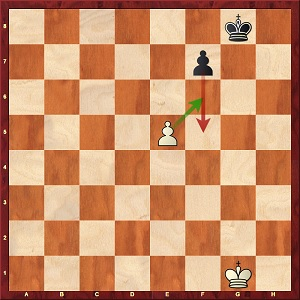
\includegraphics[scale=0.8]{img/en-passant.jpg}
\caption{Le en-passant,
\href{https://ecole.apprendre-les-echecs.com/la-prise-en-passant/}{ecole.apprendre-les-echecs.com}}
\end{figure}

L'action du en-passant ne peut en revanche être effectuée que le tour suivant l'arrivée du pion adverse à côté du premier pion. Si l'attaque n'est pas réalisée à ce moment-là alors elle n'est plus disponible pour les tours suivants.

\subsection{Les fonctions d'évaluation}\label{heuristique_contexte}
Dans l'objectif de réaliser le meilleur coup possible, il est nécessaire de définir une fonction d'évaluation permettant d'attribuer une valeur à un état du plateau de jeu afin de différencier l'efficacité des mouvements menant à la fin d'une partie.

La fonction d'évaluation est régie par une heuristique.
Une heuristique est une méthode de calcul fournissant rapidement une solution réalisable à un problème d'optimisation difficile.
\newline
Afin d'évaluer un état de plateau de jeu, nous avons pris en considération les critères définis par l'heuristique de Shannon\cite{Shannon_Heuristic}. Cette heuristique associe l'évaluation du plateau de jeu à la soustraction du plateau du joueur avec celui de son adversaire. Ainsi, pour chaque joueur, une valeur est attribuée à chaque pièce, de plus d'autres facteurs positionnels peuvent être pris en compte.
\subsubsection{Valeur des pièces}
Le principal critère de l'heuristique de Shannon est de donner une valeur à chaque pièce du plateau de jeu en fonction de l'importance des pièces. 
\newline
Les valeurs généralement utilisées sont les suivantes :
\begin{itemize}
    \item Pion : 1
    \item Cavalier : 3
    \item Fou : 3
    \item Tour : 5
    \item Dame : 9
    \item Roi : 200
\end{itemize}
Le roi possède une valeur plus élevée car il s'agit de la pièce la plus importante du plateau, puisque sa prise entraîne la fin de partie, ainsi cette valeur exprime la volonté du joueur à garder son roi, mais également à faire disparaître celui de l'adversaire.

\subsubsection{Autres critères} \label{criteres}
L'heuristique de Shannon prend également en compte des facteurs positionnels des pièces du plateau de jeu. Ces facteurs permettent de mettre en évidence des failles dans la défense des pièces ou encore la mise en place d'une tactique.
\newline

Ainsi, nous considérons l'existence de pions doublés, isolés ou encore arriérés.
\newline
Des pions doublés désignent deux pions de même couleur sur une même colonne, l'un sur une ligne au dessus de l'autre. Ce positionnement est une faiblesse pour le joueur puisque cela limite la mobilité d'un des pions et ces pions ne se protègent plus mutuellement.
\newline
Les pions isolés sont des pions qui n'ont plus de pions alliés sur les colonnes voisines. Un pion isolé est parfois considéré comme positif puisqu'il peut se transformer en pion passé permettant au pion d'obtenir une promotion. Toutefois ce positionnement rend le pion plus difficile à défendre ainsi l'heuristique de Shannon considère ce positionnement comme une faiblesse.
\newline
Un pion arriéré est un pion moins avancé que ses alliés sur les colonnes adjacentes. Ce positionnement est une faiblesse car le pion arriéré ne peut pas être défendu par ses alliés des cases adjacentes.

En raison de leurs faiblesses, l'heuristique de Shannon prévoit de soustraire 0,5 à la valeur du plateau pour chaque pion du joueur se retrouvant dans ces cas de figure et d'y ajouter 0,5 pour chaque pion de l'adversaire dans ces cas de figure.
\newline

L'heuristique de Shannon prend également en considération le nombre de coups possibles. Ainsi il faut rajouter 0,1 pour chaque mouvement possible du joueur.
\newline

Finalement, l'heuristique prend en compte l'avancement des pions. Cela se traduit par l'ajout d'une valeur de plus en plus importante au fur et à mesure que le pion se rapproche de la dernière ligne du plateau de jeu. Cela permet d'exprimer la volonté d'atteindre la dernière rangée afin d'obtenir une promotion [Voir \ref{Promotion}].

\subsubsection{Exemple de base}
\begin{figure}[h]
\centering
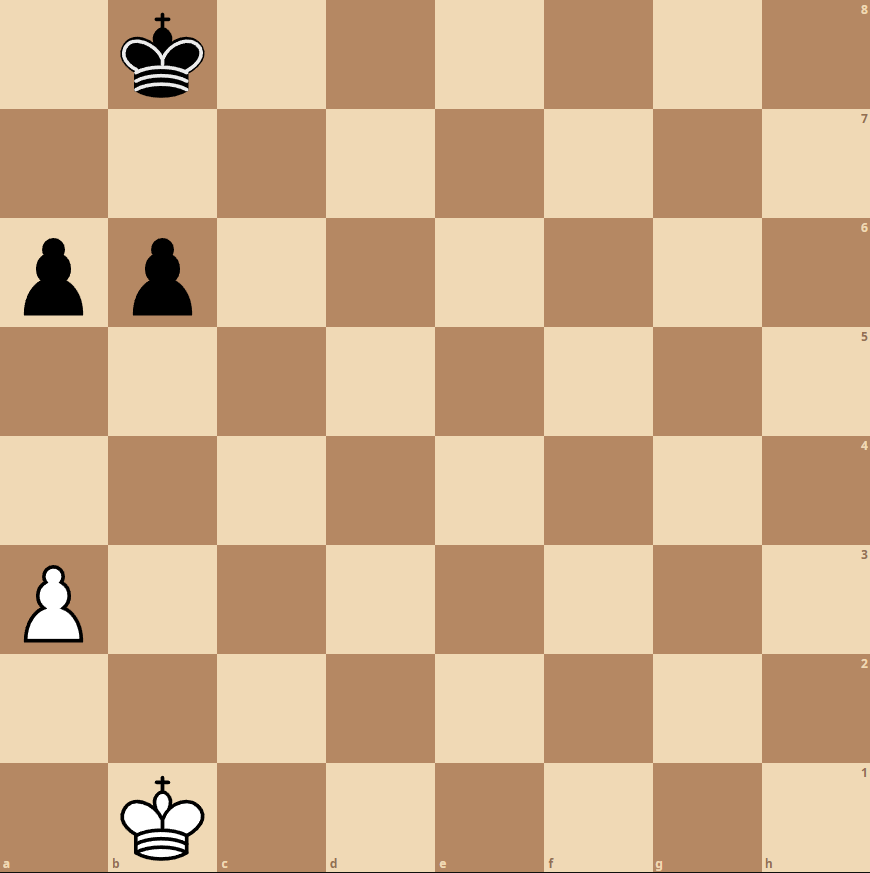
\includegraphics[scale=0.25]{img/base_heuristic.png}
\caption{Exemple de plateau, 
\href{https://lichess.org/editor/}{lichess.org}}
\end{figure}
Si nous ne considérons que la valeur des pièces, la valeur du plateau serait ici : \newline
valeur = (200 + 1) - (200 + 1 + 1) = -1 
\subsection{Génération des mouvements légaux}\label{legal_move_1.4}
Lorsque nous jouons un mouvement aux échecs, nous en choisissons un parmi les mouvements "légaux" (possible). Pour cela, il faut donc pouvoir tous les connaître avant de faire son choix.
\subsubsection{Exemple de base}
    \begin{figure}[h]
    \centering
    \includegraphics[scale=0.4]{img/mouvement_possible_pour_les_pièces_blanches.png}
    \caption{Mouvements possibles pour les pièces blanches, \href{https://lichess.org/editor/7k/8/8/8/2R1P3/8/8/6K1_w_-_-_0_1}{lichess.org}}
    \end{figure}
\newpage

\subsection{Les algorithmes de recherche}
Dans le cas de la théorie des jeux, nous utilisons des arbres de jeu, composé de noeuds représentant les positions dans un jeu. Les arêtes représentent alors les mouvements.\newline Choisir le meilleur coup revient à rechercher dans l'arbre de jeu l'heuristique la plus pertinente.

Les différents pseudo-codes associés à chaque algorithme de recherche ainsi que leur fonctionnement sont disponibles sur le net. Les algorithmes étudiés dans le cas des échecs sont :

\begin{itemize}
    \item Minimax Alpha-Beta\cite{Minmax-ab}
    \item Negamax \cite{Negamax}
    \item Negascout \cite{Negascout}
    \item MTD(f) \cite{MTD(f)}
    \item Monte-Carlo Tree Search (MCTS) \cite{MCTS}
\end{itemize}

\subsubsection{MinMax}
L'algorithme Minmax a pour objectif de trouver la liste des meilleurs coups à jouer. Pour cela, nous allons générer tous les coups possibles dans un arbre jusqu'à une certaine profondeur. Ensuite, en remontant des feuilles jusqu'à la racine, nous remontons alternativement le meilleur coup favorisant notre victoire et le meilleur coup favorisant le coup de notre adversaire.\cite{Heuristiques}.

\subsubsection{Alpha-Beta}
La variante Alpha-Beta du Minmax part du même principe mais ne prendra pas la peine de regarder certaines branches de l'arbre en effectuant un élagage. Pour cela, il utilisera deux variables, alpha et beta. Elles contiennent respectivement à chaque moment du développement de l'arbre, la valeur minimale et maximale que le joueur peut espérer obtenir pour le coup à jouer, étant donné la position où il se trouve. Ainsi, alpha et beta permettront à l'algorithme d'ignorer certaines racines de l'arbre. \cite{Heuristiques}.

\subsubsection{NegaMax}
L'algorithme Negamax se différencie de l'algorithme Minimax-ab par le fait que plutôt que maximiser le coup du joueur et minimiser le coup de l'adversaire, il inverse le signe des évaluations à chaque niveau de profondeur de l'arbre de décision et ne cherche plus qu'à maximiser la valeur du coup à évaluer\cite{Negamax}.

\subsubsection{NegaScout}
L'algorithme Négascout recherche le premier coup normalement, sur une grande profondeur, puis repère le reste des coups possibles, sur une petite profondeur, et va se demander si la valeur de alpha obtenue lors du premier coup est la meilleure.\cite{Negascout}.

\subsubsection{MTD(f)}
L'algorithme MTD(f) est basé sur la mémorisation d'un arbre de décision formée à partir de l'algorithme Minimax-ab et la formation de deux bornes, une borne supérieure et une borne inférieure. La mémorisation de l'arbre de décision permet de déterminer la valeur heuristique des coups possibles et d'effectuer un second parcours de l'arbre afin de récupérer la valeur de chaque coup et de modifier la valeur des bornes.

Le but étant de réduire l'intervalle entre les bornes jusqu'à trouver la valeur minimax correspondant au meilleur coup à jouer\cite{MTD(f)}.

\subsubsection{Monte Carlo tree search}
Avec l'algorithme Monte-Carlo Tree Search, un nœud de l'arbre de décision correspond à un état du jeu mais possède aussi deux valeurs, le nombre de simulations gagnantes et le nombre de simulations totales sur la branche.
L'algorithme fonctionne en quatre étapes\cite{MonteCarlo}:
\begin{itemize}
\item La sélection successive des enfants de la racine jusqu'à atteindre une feuille.
\item L'expansion de l'arbre, en ajoutant un enfant à la feuille si celle-ci n'est pas finale.
\item La simulation d'une partie au hasard depuis l'enfant rajouté jusqu'à atteindre une fin de partie.
\item La remontée du résultat de la partie par la mise à jour du nombre de simulations victorieuses et du nombre de simulations totales pour chaque nœud.
\end{itemize}
\subsubsection{Exemple de base}

Prenons l'exemple de l'algorithme Minmax Alpha-Beta pour expliquer en détail son fonctionnement.



\begin{figure}[!h]
\centering
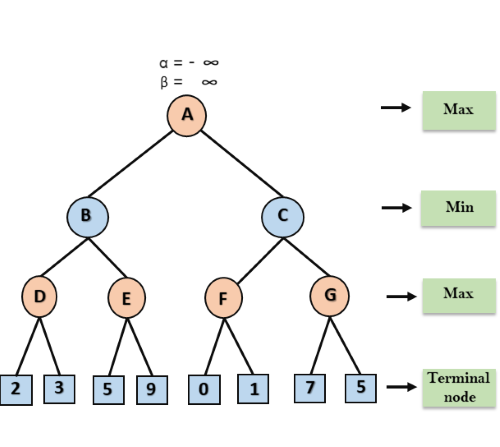
\includegraphics[scale=0.7]{img/alpha-beta-pruning-step1.png}
\caption{Première étape de l'élagage alpha-beta,
\href{https://www.javatpoint.com/ai-alpha-beta-pruning}{javatpoint.com}}
\end{figure}

En premier lieu, les variables alpha et beta sont initialisées à -$\infty$ et +$\infty$ respectivement. Elles seront ensuite passées de fils en fils, passant par le fils \textbf{b} et le fils \textbf{d}.

Sur le fils \textbf{d}, c'est la valeur de alpha qui sera modifiée car c'est au joueur max de jouer. Dans le cas présent, alpha prendra donc la valeur de 3 car max(2, 3) = 3. Le fils \textbf{d} et alpha prennent donc tous les deux la valeur 3.

\begin{figure}[!h]
\centering
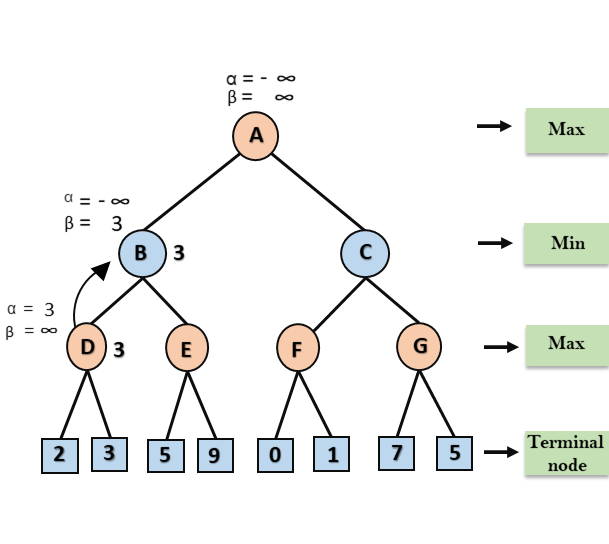
\includegraphics[scale=0.6]{img/alpha-beta-pruning-step3.png}
\caption{Poursuite de l'élagage alpha-beta,
\href{https://www.javatpoint.com/ai-alpha-beta-pruning}{javatpoint.com}}
\end{figure}

Pour le fils \textbf{b}, c'est la valeur de beta qui sera modifiée car c'est au joueur min de jouer. Dans le cas présent, beta prendra la valeur de 3 car le fils \textbf{e} n'a pas encore été étudié. Le fils \textbf{b} et beta prennent donc tous les deux la valeur 3.

Les valeurs actuelles d'alpha et beta au fils \textbf{b} sont ensuite transmises au fils \textbf{e} et le même procédé se poursuit.

\begin{figure}[!h]
\centering
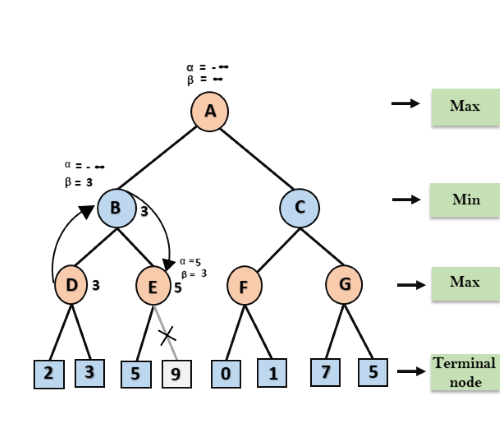
\includegraphics[scale=0.7]{img/alpha-beta-pruning-step4.png}
\caption{Poursuite de l'élagage alpha-beta,
\href{https://www.javatpoint.com/ai-alpha-beta-pruning}{javatpoint.com}}
\end{figure}

Comme alpha prendra la valeur 5, nous arriverons à une situation où alpha devient supérieur à beta. Il s'agit du signal permettant de procéder à un élagage. Il est donc inutile de regarder la feuille de valeur 9 car elle n'entraînera aucune modification pour la suite du procédé.

\begin{figure}[!h]
\centering
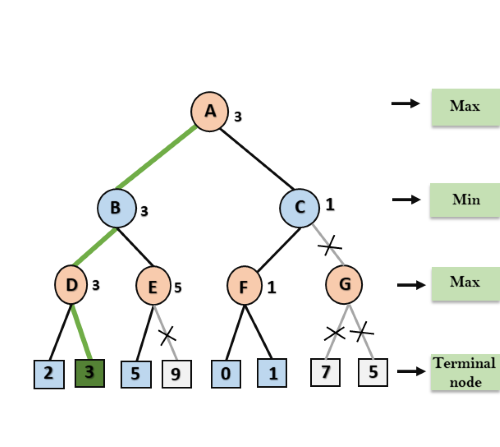
\includegraphics[scale=0.8]{img/alpha-beta-pruning-step8.png}
\caption{Arbre complet avec élagage alpha beta,
\href{https://www.javatpoint.com/ai-alpha-beta-pruning}{javatpoint.com}}
\end{figure}

En répétant les mêmes actions jusqu'au parcours complet de l'arbre, nous pouvons ainsi procéder à plusieurs élagages qui permettent d'ignorer des parties entières de l'arbre et donc de gagner du temps.

\subsection{Analyse de l'existant}
\subsubsection{Représentation du plateau de jeu}
Il existe plusieurs manières de représenter le plateau de jeu, parmi ceux ci on trouve :
L'utilisation d'un tableau à une dimension de soixante-quatre éléments, ou chaque élément correspond à une pièce (ou l'absence d'une pièce) sur une case.\newline 
L'utilisation d'un tableau à deux dimensions de taille 8x8 de manière à connaître pour chaque élément la colonne et la ligne de la case qu'il représente.\newline
Ces types de tableau peuvent contenir des entiers, des caractères ou bien des objets.\newline
Le plateau peut aussi être représenté par des structures de données contenant soixante-quatre bits, appelés bitboards. Chaque bit représente alors une case du plateau.
\subsubsection{Génération des mouvements légaux}
Les manières de générer des mouvements légaux [Voir \ref{legal_move_1.4}] sont multiples. Sans rentrer trop fortement dans les détails, nous pouvons en citer plusieurs :\newline
\begin{itemize}
    \item Tout d'abord il y a la méthode \guillemotleft naïve\guillemotright  qui est une recherche exhaustive. Suivant la position et le type d'une pièce, elle regarde pour chaque case atteignable pour ce type de pièce, si le mouvement est possible ou pas. Méthode dite aussi Brute Force.\cite{Brute_force}
    \item Il y a ensuite des méthodes utilisant les tables de recherche \cite{Lookup_table}, qui consistent à créer en amont une liste de tables prédéfinies pour les mouvements possibles de chaque type de pièce. Cette méthode est utilisable sur tout type de représentation de plateau de jeu mais plus optimisée sur les bitboards ou les tableaux à une dimension.
\end{itemize}

\subsubsection{Logiciels de jeu d'échec existants}
La plupart des logiciels de jeu d'échecs proposés au grand public, disponible dans les boutiques virtuelles comme le Microsoft Store, optent pour un affichage graphique afin de jouer aux échecs, toutefois nous pouvons se rendre compte que ces logiciels permettent aux joueurs de :

\begin{itemize}
\item sélectionner qui joue en premier. (qui joue les pièces blanches)
\item sélectionner le nombre de joueurs. (l'ia contre l'ia, 1 joueur contre l'ia ou 2 joueurs)
\item sélectionner une difficulté pour l'ia.
\item visualiser les mouvements d'une pièce.
\item sauvegarder une partie pour la reprendre plus tard. 
\item charger une partie sauvegardée.
\newline
\end{itemize}

Pour comparer avec notre projet, tout cela est possible en partie, mais notre priorité n'étant pas le jeu de l'humain contre l'humain, nous proposons avant tout une solution fortement modulable. Cette solution permet de comparer les différentes IA en temps, à profondeur égale (ou non) et avec des fonctions d'évaluation différentes. Le tout sur un grand nombre de parties pour en extraire des statistiques poussées entre les différents algorithmes disponibles.
\newline

\subsubsection{La bibliothèque "Chess" du langage Python} \label{python}
Le langage Python possède une librairie permettant de lancer un jeu d'échecs. Cette librairie permet de générer un plateau de jeu, de réaliser ou d'annuler le mouvement d'une pièce, d'afficher au format ASCII le plateau, de détecter une fin de partie ou encore de détecter les répétitions de mouvements.

\subsubsection{Évènements majeurs des logiciels d'échec}

Il existe également des logiciels, quant-à eux plus scientifiques, avec pour vocation d'exercer des algorithmes contre des champions humains ou contre d'autres logiciels.
\newline
C'est le cas de Kaissa qui fût le premier programme à avoir gagné le championnat ACM d'échecs informatiques de 1974. Ce dernier utilise un algorithme Minimax alpha beta \cite{KaissaAB} pour calculer ses coups et un système de bitboards pour déterminer les mouvements légaux d'une pièce. \cite{Kaissa}\cite{KaissaBitboard}\cite{RotatedBitBoards}.
\newline
Nous pouvons citer Deep Thought qui remporta le 19ème championnat ACM d'échecs informatiques, il s'agit du premier ordinateur avec le niveau d'un grand maître qui joua contre Garry Kasparov en 1989 et fut battu.\cite{Deep}. 
\newline
Jusqu'à Deep Blue, doté d'une architecture massivement parallèle, lui permettant de paralléliser l'algorithme de recherche alpha-bêta\cite{DeepSystem} et fut le premier ordinateur à avoir battu Kasparov en 1996.\cite{Deep}.

\section{Description des besoins}

\subsection{Besoins fonctionnels}
\medskip

\begin{enumerate}
    \item Conserver le plateau de jeu \hfill[Implémenté]
    \medskip
    \item Charger le plateau de jeu \hfill[Implémenté]
    \medskip
    \item Afficher le plateau de jeu \hfill[Implémenté]
    \medskip
    \item Générer les mouvements des pièces non-glissantes \hfill[Implémenté]
    \medskip
    \item Générer les mouvements des pièces glissantes \hfill[Implémenté]
    \medskip
    \item Générer les mouvements des coups spéciaux \hfill[Non-Implémenté]
    \medskip
    \item Jouer un coup \hfill[Implémenté]
    \medskip
    \item Conserver un historique des coups \hfill[Implémenté]
    \medskip
    \item Défaire un coup \hfill[Implémenté]
    \medskip
    \item Détecter une victoire \hfill[Implémenté]
    \medskip
    \item Détecter un match nul \hfill[Implémenté]
    \medskip
    \item Sélectionner un algorithme \hfill[Implémenté]
    \medskip
    \item Sélectionner une fonction d'évaluation \hfill[Implémenté]
    \medskip
    \item Jouer contre un algorithme \hfill[Implémenté]
    \medskip
    \item Organiser une partie \hfill[Implémenté]
    \medskip
    \item Générer un récapitulatif de match \hfill[Non-Implémenté]
    \medskip
    \item Lancer un tournoi entre algorithmes \hfill[Non-Implémenté]
    \medskip
    \item Confronter des algorithmes à des énigmes \hfill[Non-Implémenté]
    \medskip
\end{enumerate}

\subsubsection{Conserver le plateau de jeu}
\medskip
\begin{itemize}
    \item Le plateau est conservé à l'aide de bitboards \cite{Bitboards}, chaque bitboard représente l'emplacement des pièces d'un même type et d'une même couleur. Il y a un bitboard pour l'emplacement de tous les pions blancs, un bitboard pour l'emplacement de tous les cavaliers blancs,...).
\end{itemize}
\newpage
\subsubsection{Charger le plateau de jeu}
\begin{itemize}
    \item Le plateau de jeu peut être chargé à partir d'une chaîne de 64 caractères, chaque caractère correspond à une case.
\end{itemize}
\medskip
\medskip
\subsubsection{Afficher le plateau de jeu}
\medskip
\begin{itemize}
    \item Affichage en texte, une lettre représente un pion (p = pion, k = roi, q = reine,
    b = fou, r = tour, n = cavalier).
    Les cases vides, quand à elles contiendront un point "." dans un souci de lisibilité.
    \item Afin de différencier les pions des 2 joueurs du plateau de jeu, le joueur blanc aura des pions en majuscules et le joueur noir en minuscules.
    \item Les coordonnées des cases seront les mêmes que sur le jeu d'échecs original, les numéros représentent les lignes et les lettres pour les colonnes, par exemple (a1 = 1ère case en bas à gauche \dots).
\end{itemize}
\begin{figure}[h]
\centering
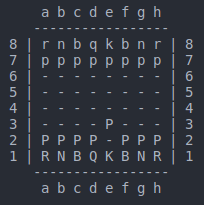
\includegraphics[scale = 0.5]{img/pdp_chess_board.png}
\caption{Plateau de jeu en version texte réalisé par nos soins}
\end{figure}
\medskip
\subsubsection{Générer les mouvements des pièces non-glissantes}
\begin{itemize}
    \item Le programme doit pouvoir générer les mouvements de toutes les pièces non-glissantes.
    \item Ces mouvements doivent prendre en compte la position des autres pièces.
\end{itemize}
\medskip
\subsubsection{Générer les mouvements des pièces glissantes}
\begin{itemize}
    \item Le programme doit pouvoir générer les mouvements de toutes les pièces glissantes.
    \item Ces mouvements doivent prendre en compte la position des pièces qui pourraient bloquer leurs lignes de déplacements.
\end{itemize}
\medskip
\subsubsection{Générer les mouvements des coups spéciaux}
\begin{itemize}
    \item Le programme doit être capable de générer les différents coups spéciaux existants si les conditions sont réunies.
    \item Il doit être capable de générer le roque, le en-passant et la transformation.
\end{itemize}
\medskip
\subsubsection{Jouer un coup}
\begin{itemize}
    \item Le programme doit pouvoir appliquer un coup sur le plateau.
    \item Le coup n'est pas vérifié avant application, car il ne doit être possible de jouer qu'un coup généré par le moteur de jeu lui-même.
\end{itemize}

\medskip
\subsubsection{Conserver un historique des coups}
\begin{itemize}
    \item Le programme doit conserver en mémoire tout les coups joués.
    \item Il doit être possible d'ajouter ou d'enlever un coup de cet historique.
\end{itemize}
\medskip
\subsubsection{Défaire un coup}
\begin{itemize}
    \item Le programme doit être capable de défaire un coup à l'aide de l'historique.
    \item La modification doit être appliquée sur le plateau de jeu.
\end{itemize}
\medskip
\subsubsection{Détecter une victoire}
\begin{itemize}
    \item Le programme doit être capable de vérifier si un plateau donné entraîne la victoire de l'un des deux joueurs.
    \item Le programme doit arrêter le match une fois cette victoire détectée et annoncer le vainqueur sur la console.
\end{itemize}
\medskip
\subsubsection{Détecter un match nul}
\begin{itemize}
    \item Le programme doit être capable de vérifier si un plateau donné entraîne un match nul.
    \item Le programme doit arrêter le match une fois ce match nul détecté et l'annoncer sur la console.
\end{itemize}
\medskip
\subsubsection{Sélectionner un algorithme}
\begin{itemize}
    \item Il doit être possible de sélectionner un algorithme parmi ceux existants.
    \item L'algorithme doit pouvoir être utilisé dans le moteur de jeu.
    \item L'algorithme doit être paramétrable.
\end{itemize}
\medskip
\subsubsection{Sélectionner une fonction d'évaluation}
\begin{itemize}
    \item Le programme doit permettre de sélectionner différents paramètres afin de personnaliser la fonction d'évaluation.
    \item La fonction d'évaluation doit être utilisable par un algorithme.
\end{itemize}
\medskip
\subsubsection{Jouer contre un algorithme}
\begin{itemize}
    \item Le programme doit permettre à deux algorithmes de jouer l'un contre l'autre.
    \item Le programme doit permettre à un joueur humain de jouer contre un algorithme.
    \item Le programme doit avoir un joueur de type aléatoire.
\end{itemize}
\medskip
\subsubsection{Organiser une partie}
\begin{itemize}
    \item Le programme doit être capable, à partir d'un fichier de configuration, d'organiser une partie complète entre deux joueurs.
    \item Le fichier de configuration doit contenir tout les paramètres d'un algorithme.
    \item Le fichier de configuration doit contenir tout les paramètres d'une heuristique et l'associer à un algorithme.
\end{itemize}
\medskip
\subsubsection{Générer un récapitulatif de match}
\begin{itemize}
    \item Le programme doit pouvoir générer un fichier contenant toutes les données d'une partie.
    \item Les paramètres des joueurs.
    \item Les coups joués.
    \item Le résultat du match.
    \item Le temps d'exécution.
\end{itemize}
\medskip
\subsubsection{Lancer un tournoi entre algorithmes}
\begin{itemize}
    \item Le programme doit être capable d'organiser un tournoi à partir d'un fichier de configuration.
    \item Le tournoi serait une forme de "ligue" où chaque algorithme jouerait 2 fois contre tous les autres, une fois en tant que joueur blanc une fois en tant que joueur noir.
    \item Le programme doit être capable de générer un classement de tous les algorithmes suivant le nombre de victoires et suivant le nombre de coups joués jusqu'à la victoire.
\end{itemize}
\medskip
\subsubsection{Confronter des algorithmes à des énigmes}
Dans le monde des échecs, il existe des "problèmes" d'échec \cite{Krt}, c'est à dire d'après un plateau donné, il faut réussir à mettre en place des stratégies comme mettre le roi adverse en échec et mat en un certain nombre de coups.
\begin{itemize}
    \item Le programme doit générer une partie suivant ce format.
    \item Il doit être possible de configurer les algorithmes à utiliser sur cette énigme.
    \item Les énigmes sont stockées dans le dossier énigmes dans un fichier au nom de l'énigme.
    \item Dans les fichiers énigmes/*, à la suite de l'échiquier de départ se trouve les conditions de victoires de l'énigme : "EM" pour un échec et mat, "EMC5" Si il faut un échec et mat en moins de 5 coups \dots
\end{itemize}
\begin{figure}[!h]
        \centering
        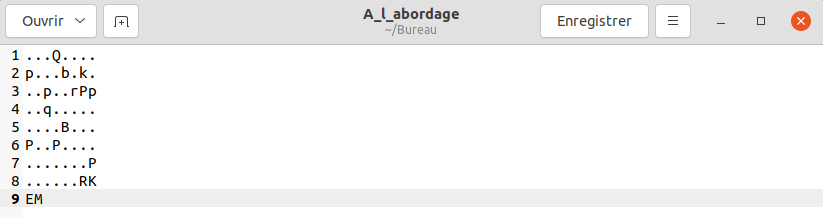
\includegraphics[scale = 0.3]{img/a_l_abordage.png}
        \caption{Exemple d'un fichier énigme réalisé par nos soins}
        \label{fig:enigm}
    \end{figure}
\medskip
\subsection{Besoins non-fonctionnels}
\medskip
\subsubsection{Performances}
Le programme doit répondre rapidement aux commandes utilisateurs.
Le moteur de jeu doit être au moins aussi performant que la bibliothèque chess de python \ref{python}.
\medskip
\subsubsection{Fiabilité}
Il ne doit pas y avoir d'erreurs lors de l'exécution du programme. 
Les commandes utilisateur ainsi que la lecture du fichier de configuration doivent être robustes.
\medskip
\subsubsection{Facilité d'utilisation} 
Toutes les commandes possibles doivent être listées à l'utilisateur, ainsi que leurs fonctions, afin de le guider et qu'il ne perde pas de temps à comprendre le fonctionnement du programme.
La configuration d'une partie doit être documentée pour permettre à l'utilisateur de la modifier ou d'en créer une autre.
\medskip
\subsubsection{Domaine d'action} 
Les utilisateurs seront des informaticiens. Le programme étant basé avant tout sur l'interaction d'une IA contre une autre. 
Une partie entre un humain et une IA est totalement possible.
\medskip
\subsubsection{Portabilité} 
Le programme doit être exécutable sous les systèmes d'exploitation suivants : Ubuntu 20.04 et Ubuntu 21.10.

\newpage
\section{Architecture}

\subsection{Points Techniques d'implémentation}
Notre programme ne gère pas le multi-threading.

\subsubsection{Le langage}

Nous avons choisi d'utiliser le langage c++ pour ce projet. En effet celui-ci nous paraissait le plus adapté par rapport à nos deux objectifs d'implémentation principaux :
\begin{itemize}
    \item L'optimisation des ressources mémoire et de calcul.
    \item Une architecture orientée objet.
\end{itemize}
Ce langage nous permet d'utiliser des structures de données légères, et grâce à l'utilisation de références et pointeurs de les passer aux différentes parties du code sans les copier.
Il nous permet également d'utiliser l'héritage et le polymorphisme, éléments clés d'une architecture orientée objet.

\subsubsection{Les bitboards}
Nous avons choisi la technique des bitboards [Voir \cite{Bitboards}] pour représenter nos différents plateaux de jeu.
Cette représentation possède l'avantage d'être très légère et de permettre certains types de calculs particulièrement rapides mais présente aussi plusieurs inconvénients.
Dans notre projet, un bitboard est encodé par un uint64\_t ainsi qu'un char, ce qui correspond à un entier non-signé de 64 bits et un entier de 8 bits.
L'ajout de ce caractère nous permet d'associer efficacement un bitboard à la pièce qu'il représente. [Voir \ref{implementation_plateau}]
\paragraph{Calculs sur les bitboards} \label{calculs_sur_les_bitboards}
~~\\
Nous opérons sur les bitboards avec des opérations dites bit à bit, elles consistent en la transformation de l'état d'un ou plusieurs bits dans notre structure de données.
On y retrouve les opérations logiques du type NOT, OR, AND, ainsi que les opérations de décalage des bits à gauche ou à droite.
Grâce à ces opérations élémentaires, nous formons des opérations plus complexes :
\begin{itemize}
    \item \textbf{Les filtres : }
    Ces opérations utilisent des bitboards pour en former un nouveau, nous utilisons ce type d'opération pour générer des bitboards de positions atteignables ou bien de positions bloquées par des alliés. 
    \item \textbf{Les requêtes : }
    Ces opérations utilisent des bitboards pour récupérer une ou plusieurs valeurs, nous les utilisons pour vérifier la présence d'un bit à un certain index, ou bien pour obtenir la position des bits actifs.
\end{itemize}

\paragraph{Détection des bits actifs}
~~\\
\newline
La détection des bits actifs est une opération importante dans le projet, car elle nous permet d'obtenir les index de chaque bit actif et donc d'itérer sur ces positions pour réaliser d'autres opérations. C'est pour cela que nous en avons réalisé deux versions.
\subparagraph{Recherche exhaustive} \label{recherche_bit_exhaustive}
~~\\
\newline
C'est une version naïve qui itère sur chaque bit et vérifie s'il est actif, la vérification est peu coûteuse mais l'algorithme itère toujours 64 fois. 
\subparagraph{Recherche par soustraction} \label{recherche_bit_soustraction}
~~\\
\newline
Une version plus coûteuse en ressources mais qui a l'avantage de n'itérer que le même nombre de fois que le nombre de bits actifs. Celle-ci parait plus intéressante dans la mesure où les bitboards sur lesquels nous itérons ne dépassent jamais 8 bits actifs, c'est le bitboard des pions d'une couleur sans qu'aucun d'entre eux ne soit pris.\newline
Nous verrons par la suite le résultat de leur comparaison [Voir \ref{resultats_moteur}]

\newpage
\subsubsection{Les mouvements}\label{Mouvements}
Les mouvements sont une structure contenant plusieurs informations sur un coup joué ou jouable.
A savoir : 
\begin{itemize}
    \item \textbf{La position de départ} (index du bit où se situe la position de départ ).
    \item \textbf{Le type de pièce qui bouge} (sous forme d'un char ('P' pour un pion blanc, 'p' pour un pion noir etc \dots).
    \item \textbf{La position d'arrivée}  (index du bit où se situe la position d'arrivée).
    \item \textbf{Le type de pièce de la case d'arrivée} ('-' si aucune pièce n'est présente) cela permet de savoir si une pièce adverse a été mangée durant le mouvement et si oui, laquelle.
\end{itemize}

\subsubsection{La génération des mouvements légaux}
Pour pouvoir générer des mouvements, nous avons besoin de savoir où nos pièces peuvent aller.
Pour cela, nous avons besoin de détecter toutes les positions atteignables par les pièces du joueur à qui c’est le tour de jouer, ainsi que de vérifier si ces positions atteignables sont jouables, par rapport à un plateau donné.
Nous avons deux versions bien différentes qui répondent à ce besoin.

\paragraph{Version 1} \label{mouvements_legaux_v1}
~~\\
\newline
Dans un premier temps nous sommes partis sur une version brute force et générique des mouvements légaux, ne prenant pas en compte le fait d’utiliser correctement les bitboards \cite{Bitboards} et leurs opérations.
Nous avons donc cherché les positions atteignables pour chaque pièce une à une.

\subparagraph{A la volée}
~~\\
\newline
Pour chaque type de pièce, nous avons une fonction qui va itérer sur chaque pièce du même type et de la couleur du joueur (noir ou blanc), et qui va chercher toutes les positions atteignables par celui-ci ainsi que vérifier si elles sont aussi réalisables suivant les pré-conditions requises.
On va donc faire cas par cas la recherche et les vérifications avant de créer le mouvement légal.
Par exemple, pour le pion blanc nous allons regarder les quatre positions atteignables qui sont avancées d'une case, avancées de deux cases, manger en diagonale à droite d'une case et manger en diagonale à gauche d'une case (exemple sur l'avancement d'une case, il suffit de faire +8 à l'index de départ).
Ensuite sur chaque index de position atteignable, nous vérifions les pré-conditions (exemple sur l'avancement d'une case, vérifier qu'il n'y a pas une pièce adverse ou alliée à la position atteignable, autre exemple pour manger à droite ou à gauche, vérifier qu'il y a une pièce adverse à la position atteignable).

\paragraph{Version 2} \label{mouvements_legaux_v2}
~~\\
\newline
Dans un second temps, nous avons fait une version des mouvements légaux en utilisant au maximum les bitboards et leurs opérations.
Pour cela, nous avons une première approche légèrement différente pour les pièces dites non glissantes.
\subparagraph{A l'aide de tables de correspondance} \label{tables_de_correspondances}
~~\\
\newline
A la création du jeu, pour les pièces non glissantes (roi, pion, cavalier) nous générons dans des lookuptable (table de bitboards) les positions atteignables selon la position de départ (par exemple pour les cavaliers nous avons 64 bitboards qui correspondent chacun aux positions atteignables par un cavalier selon sa position de départ, le premier bitboard correspond aux positions atteignables pour une position de départ à l'index zéro).\newline
Les lookuptable pour les pions étaient les plus difficiles à réaliser car il s'agit de la seule pièce que ne mange pas de la même façon qu'elle se déplace et les déplacements des pions blanc sont différents des déplacements des pions noirs (graphiquement les pions blancs "montent" alors que les pions noirs "descendent"). \newline
De plus, elle possède un mouvement spécial en début de partie (quand elle est sur sa position de départ, elle peut avancer d'une seule ou deux cases).\newline
Nous avons donc une lookuptable pour pions blancs et une lookuptable pour les pions noirs.\newline
De plus, nous avons séparé chacune d'elles en 2 parties, une partie pour les tables de mouvements et l'autre pour les d'attaques.\newline
En utilisant cette méthode, nous n'avons plus besoin de recalculer les positions atteignables pour ces pièces, il nous suffira d'aller chercher nos positions atteignables dans les lookuptable et de leur appliquer ce que nous allons définir en suivant comme "des masques", pour vérifier si ces positions sont jouables.

\subparagraph{A l'aide de masques}
~~\\
\newline
Nous allons utiliser des filtres [Voir \ref{calculs_sur_les_bitboards}] (opérations entre bitboards) qui vont sortir des masques (résultat d'un filtre sous forme d'un bitboard)
contenant les positions jouables pour un type de pièce et une position de départ.\newline
Cette technique sera utilisée tout le long de la génération des mouvements légaux pour les pièces glissantes alors que pour les pièces non-glissantes, elle sera utilisée que pour vérifier si une position atteignable est jouable.\newline
Exemple pour le cavalier (pièce non glissante), nous récupérons nos positions atteignables par rapport à notre position de départ dans le lookuptable [Voir \ref{tables_de_correspondances}] correspondant et nous appliquons l'opération logique AND entre ce dernier et le bitboard correspondant aux emplacements où il n'y a pas de pièce alliée.

\subsubsection{L'historique} \label{L'historique}
Nous gardons en mémoire l'historique des mouvements joués dans un vecteur.\newline
Ce vecteur fonctionne comme une pile, c'est à dire que nous allons ajouter les mouvements joués un à un dans l'ordre dans lequel ils ont été joués, et lorsque nous récupérons un mouvement, nous récupérerons le dernier mis dans ce vecteur, donc le dernier joué.

\subsubsection{Le plateau} \label{implementation_plateau}
Pour contenir l'entièreté du plateau, il est nécessaire de définir un bitboard pour chaque type de pièce et chaque couleur, ce qui revient à en stocker 12 (6 type de pièces * 2 couleurs).
A cela s'ajoute 2 bitboards supplémentaires contenant l'ensemble des pièces pour chaque couleur, ces 2 bitboards sont mis à jour à chaque déplacement ou prise de pièce.
Ils permettent d'effectuer des opérations de présence de pièces sans avoir à itérer sur tout les bitboards. \newline
C'est également le plateau qui contient l'historique, ainsi que les vérifications des conditions d'arrêt.

\subsubsection{La fonction d'évaluation}\label{heuristique_architecture}
\paragraph{Les critères d'évaluation}
~~\\
\newline
Pour ne pas travailler sur des nombres flottants, nous avons multiplié les valeurs de défaut, définies grâce à l'heuristique de Shannon, par 20 ainsi la valeur heuristique de l'avancement d'un pion passe de 0,05 à 1.

\paragraph{Les valeurs des pièces}
~~\\
\newline
Nous nous sommes tout d'abord penchés sur l'attribution d'une valeur à chaque pièce du plateau de jeu. Pour cela, nous récupérons l'ensemble des bitboards qui constitue l'ensemble des pièces du joueur, que nous sélectionnant via sa couleur. Nous partons d'une valeur de plateau à valeur 0.\newline

Pour chaque bitboard récupéré, nous le parcourons et comptons le nombre de bits à valeur 1. Ce nombre est alors multiplié par la valeur définie dans l'heuristique correspondant à son type. Ainsi en utilisant un plateau de jeu constitué de 8 pions et un roi et avec les valeurs heuristiques par défaut, en d'autres termes si nous attribuons la valeur 20 aux pions et 4000 au roi, le parcours du bitboard correspondant aux pions renvoie la valeur 20 et celui correspondant au roi renvoie 4000 donnant une valeur de plateau de 4020.
\newline
\paragraph{Les facteurs positionnels}
~~\\
\newline
Puis nous avons réalisé l'implémentation des facteurs positionnels.\newline 
Comme ces facteurs ne concernent que la position des pions, nous ne récupérons que le bitboard correspondant aux pions.\newline

Pour compter le nombre de pions doublés, nous parcourons le bitboard des pions et lorsque nous tombons sur un bit à valeur 1, nous vérifions si le bit correspondant à la case en dessous à pour valeur 1.\newline
Si tel est le cas, nous incrémentons le nombre de pions doublés.\newline

Pour compter le nombre de pions isolés, nous parcourons le bitboard des pions et lorsque nous tombons sur un bit à valeur 1, nous supposons qu'il s'agit d'un pion isolé puis nous vérifions les bits correspondant aux colonnes adjacentes et de sa propre colonne, si nous rencontrons un bit à valeur 1 sur les colonnes parcourues nous mettons à jour le fait que le pion est isolé et arrêtons le parcours des colonnes pour chercher un autre pion potentiellement isolé. Si tel n'est pas le cas, nous incrémentons le nombre de pions isolés.\newline

Pour compter le nombre de pions arriérés, nous parcourons le bitboard des pions et lorsque nous tombons sur un bit à valeur 1, nous supposons qu'il n'est pas arriéré puis nous vérifions si les cases plus avancées d'une ligne sur les colonnes adjacentes sont occupées par un pion. Si c'est le cas, nous supposons qu'il est arriéré puis nous vérifions les cases les moins avancées d'une ligne sur les colonnes adjacentes, s'il y a un pion à l'un de ces emplacements alors nous mettons à jour l'information que le pion n'est pas arriéré. Et à la fin de ces processus si notre information indique que le pion rencontré est arriéré nous incrémentons alors le nombre de pions arriérés.

Lorsque nous récupérons le nombre de pions, correspondant à un des facteurs positionnels, nous le multiplions par sa valeur heuristique avant de soustraire à la valeur du plateau du joueur le résultat obtenu, puisqu'il s'agit de facteurs considérés comme défavorables au joueur.
\newline

Tout ce processus nous permet ainsi d'obtenir une valeur de plateau du joueur. Nous les répétons afin d'obtenir une valeur du plateau de l'adversaire que nous soustrayons au plateau du joueur.

\paragraph{Le facteur de mobilité}
~~\\
\newline
Nous nous sommes intéressés au facteur de mobilité.\newline
La liste des mouvements légaux possibles [Voir \ref{Mouvements}] étant récupérable,
Le nombre d'éléments dans cette liste correspond au nombre de mouvements légaux possibles.
Nous multiplions ce nombre par sa valeur définie dans l'heuristique que nous ajoutons à la valeur du plateau de jeu.\newline
Nous répétons cette action pour chaque bitboard constituant le plateau du joueur.

\paragraph{L'avancement d'un pion}
~~\\
\newline
Nous avons ensuite implémenté l'avancement des pions. Pour chaque pion, nous récupérons sa position puis nous déterminons la ligne sur laquelle il se positionne puis nous multiplions la ligne par la valeur de mobilité, définie dans l'heuristique, avant de l'ajouter à la valeur du plateau du joueur. Nous répétons ce processus pour les pions adverses à la différence qu'au lieu d'ajouter la valeur de l'avancement du pion adverse nous la soustrayons à la valeur du plateau du joueur. 
\paragraph{La modularité}
~~\\
\newline
Dans la situation où la valeur d'un critère est égale à 0 alors l'évaluation de ce critère sera omis.
Cela permet à la fonction d'évaluation de ne pas perdre en performance malgré la présence ou non de l'évaluation d'un critère. 

\subsubsection{Les joueurs}\label{player_architecture}

\paragraph{Les algorithmes}
~~\\
\newline
Nos algorithmes sont tous dépendants de la profondeur, nous n'avons pas de contraintes de temps d'exécution. \newline
Les algorithmes que nous avons implémentés sont originellement déterministes du fait de l'ordre des mouvements légaux qu'ils reçoivent. En effet, cet ordre sera toujours identique pour un plateau de jeu donné. 
Nous avons décidé d'ajouter un mélange de ces mouvements légaux avant leurs traitements, ce qui permet une plus grande variété de plateau de jeu. Ce mélange conserve l'optimalité des algorithmes pour une heuristique donnée et à une profondeur de recherche donnée, mais les rend non déterministes.
Finalement tout nos algorithmes ont une optimisation du nombre de noeuds parcourus par rapport à l'algorithme MinMax.

\paragraph{Humain}
~~\\
\newline
Le joueur humain permet à un utilisateur d'interagir avec le moteur de jeu depuis la console.
Il affiche la liste des coups possibles et attend la réponse sur la console.

\paragraph{Aléatoire}
~~\\
\newline
Le joueur aléatoire mélange la liste des mouvements légaux et joue le premier mouvement de celle-ci.
Il est utile pour vérifier la validité des autres algorithmes.

\subsubsection{Jouer un coup}\label{domove}
Jouer un coup consiste à appliquer un mouvement à notre plateau, c'est à dire que dans le bitboard correspondant au type de la pièce qui effectue le mouvement, nous allons mettre le bit ayant comme index la position de départ à 0 et le bit qui a pour index la position d'arrivée à 1.\newline 
Nous vérifions aussi si ce mouvement correspond à une attaque, donc s'il mange une pièce.\newline
Dans le cas d'une prise de pièces, le bitboard correspondant au type de la pièce mangée se voit retirer le bit qui a pour index la position d'arrivée.\newline
Lorsque nous jouons un coup, nous enregistrons le mouvement dans l'historique [Voir \ref{L'historique}].\newline
Nous avons aussi la possibilité de "défaire un coup" grâce à l'historique, nous récupérons le dernier coup joué dans l'historique et nous appliquons l'inverse de jouer un coup en vérifiant si ce coup n'avait pas mangé une pièce, auquel cas nous la faisons réapparaître.

\subsubsection{Les conditions d'arrêt} \label{Architecture_condition_d'arrêt}
Le jeu est fini lorsque l'un des deux joueurs a gagné, donc le joueur blanc a gagné s'il a réussi à manger le roi du joueur noir et inversement.\newline
Le jeu s'arrête aussi s'il y a match nul, pour cela il peut y avoir plusieurs raisons :
\begin{itemize}
    \item Si cinquante coups ont été effectués à la suite sans capture.\newline
    Pour cela, nous allons vérifier dans l'historique [Voir \ref{L'historique}] les cinquante derniers coups, regarder si le type de la position d'arrivée est une pièce ou non et incrémenter un compteur si un coup n'a pas mangé ainsi que de le remettre à zéro sinon.
    \item Si les deux joueurs ne peuvent plus se mettre en échec et mat car ils ne possèdent pas les pièces nécessaires.\newline
    Ces cas sont, si les deux deux joueurs possèdent plus que leur roi, si l'un possède plus que un roi et un fou et l'autre uniquement son roi, si l'un possède plus que un roi et un cavalier et l'autre uniquement son roi ou si les deux joueurs n'ont plus que leur roi et un fou.\newline
    Pour cela, nous vérifions si les bitboards de toutes les pièces correspondent à l'un de ces cas (exemple bitboard pièces blanches correspond au bitboard des rois blancs et bitboard pièces noires correspond au bitboard des rois noirs, etc \dots).
    \item Si le plateau apparaît trois fois dans la partie.\newline
    Nous l'avons géré un peu différemment, nous sommes partis du principe que deux plateaux identiques sont séparés d'au moins quatre coups (joueur blanc bouge une pièce (1), joueur noir bouge une pièce (2), joueur blanc remet sa pièce en position initiale (3), joueur noir remet sa pièce en position initiale(4) ).\newline
    Donc pour chaque plateau, grâce à l'historique, nous regardons si le plateau d'il y a quatre coups et celui d'il y a huit coups sont identiques à notre plateau courant.
\end{itemize}

\subsubsection{Le jeu}
Notre boucle de jeu se situe dans la classe "Game" qui elle contient les deux joueurs [Voir \ref{player_architecture}], à l'intérieur se situe la boucle principale qui s'arrêtera selon les conditions d'arrêt [Voir \ref{Architecture_condition_d'arrêt}].\newline
À chaque tour de boucle, nous récupérons le joueur à qui c'est le tour de jouer, celui-ci va nous donner le coup qu'il veut jouer ( son meilleur coup selon lui ), et nous appliquons ce coup [Voir \ref{domove}] au plateau.\newline
À la fin de la boucle, nous changeons le joueur courant, afin qu'au tour suivant, ce soit à l'autre de jouer. \newline

\subsubsection{La préparation d'un match}
\paragraph{La configuration}
~~\\
\newline
Nous avons donc décidé d'utiliser des fichiers json pour le passage de paramètres des parties.
Afin d'utiliser les fichiers json pour la création des parties, ainsi que des IA, il est nécessaire d'avoir la librairie jsoncpp, disponible à l'adresse suivante \cite{JsonCpp}.\newline
Cela donne certains avantages, il n'y as pas besoin de recompiler le programme pour lancer des parties différentes, avec des joueurs différents ainsi que des paramètres ou heuristiques différentes, pour cela il suffit de modifier le fichier json que le programme lit.
\newpage
\begin{figure}[!h]
    \centering
    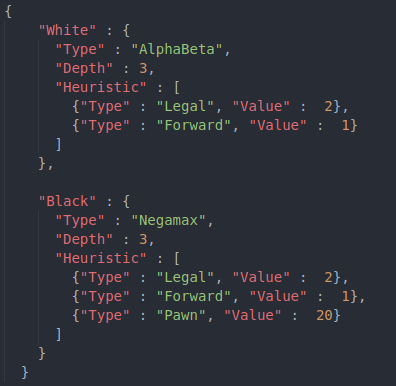
\includegraphics[scale = 0.7]{img/fichierjson.png}
    \caption{Illustration d'un fichier json de PDP CHESS}
    \label{json}
\end{figure}


Une hiérarchie sera présente sur les fichier Json de la manière suivante:
\begin{enumerate}
    \item \textbf{Les Couleurs des joueurs :} White, Black.
    \item \textbf{Le type des deux joueurs / IA, ainsi que leurs paramètres si IA :}
    \begin{itemize}
        \item \textbf{Le type :} AlphaBeta, Negamax, Negascout \dots
        \item \textbf{La profondeur :} La profondeur de recherche de l'IA.
        \item \textbf{L'heuristique :} 
        \begin{itemize}
            \item \textit{Les personnalisations d'heuristique possible :} Nous pouvons mettre des poids à certaines options (Par exemple \{"Type" : "Legal", "Value" :  2\} met un poids de 2 sur le nombre de mouvements légaux disponible à un joueur [voir \ref{Mouvements}]. Plus ce poids est haut, plus l'IA va chercher à ouvrir son jeu pour avoir davantage de possibilités de coups disponibles.)\newline
            Si aucun paramètre n'est donné à l'heuristique, une heuristique par défaut sera générée.
        \end{itemize}
    \end{itemize}
   
\end{enumerate}

\paragraph{Les paramètres}
~~\\
\newline
Les paramètres sont des structures qui représentent les différents éléments configurables dans le fichier json.
En faire des structures permet d'ajouter un degré de vérification sur les valeurs et type de la configuration, mais aussi de préparer une potentielle réutilisation de ceux-ci pour une récupération des paramètres dans un autre format de stockage tel le csv.  

\subsubsection{La fabrique}
La fabrique permet d'instancier tout les joueurs, elle ajoute un degré de résilience à la génération des joueurs en générant un joueur de type aléatoire si la lecture du fichier json a rencontré une erreur.

\subsubsection{Le directeur}
Le directeur sert de passerelle entre l'utilisateur et l'ensemble du projet, il instancie tout les composants nécessaires au bon déroulement d'une ou plusieurs parties.
Il est résilient aux fichiers qui ne sont pas lisibles par la bibliothèque jsoncpp, et jusqu'à un certain point à une mauvaise écriture des fichiers json.

\newpage
\subsection{Diagrammes}
\subsubsection{Diagramme de paquetage}
\paragraph{Engine}
~~\\
\newline
Le paquetage Engine du logiciel est toute la partie du moteur de jeu.\newline 
Elle gère donc tout ce qui est fonctionnement de base du jeu d'échec, c'est à dire : 
\begin{itemize}
    \item Générer un plateau de jeu avec une configuration particulière.
    \item Appliquer un mouvement donné au plateau de jeu.[Voir \ref{domove}]
    \item Garder en mémoire les différents mouvements appliqués durant la partie en cours.
    \item Retirer le dernier mouvement appliqué.
    \item Dire si un plateau est en situation de fin de jeu. [Voir \ref{condition d'arret}]
\end{itemize}
Pour faire cela, il est composé des sous-paquetages suivants :

\subparagraph{Board}
~~\\
\newline
\begin{figure}[!h]
    \centering
    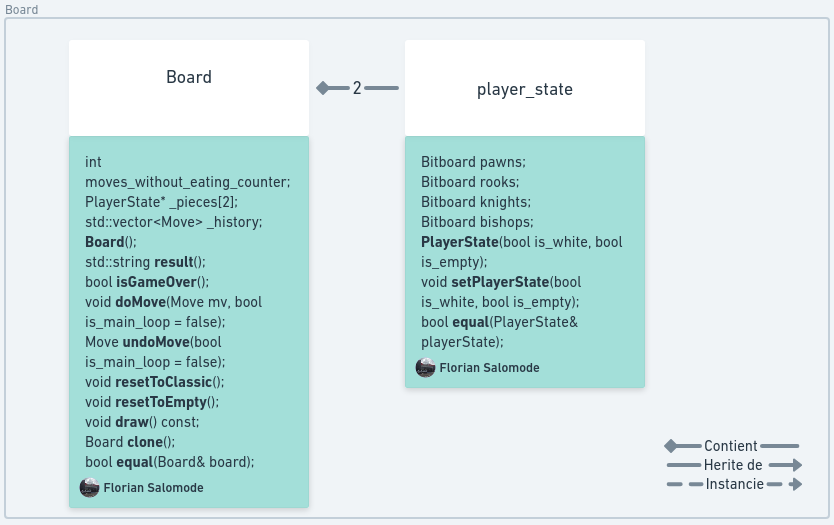
\includegraphics[scale = 0.4]{img/Package/Board.png}
    \caption{Paquetage Board de PDP CHESS}
    \label{pck:board}
\end{figure}

Le paquetage Board représente l'abstraction de notre plateau de jeu, ainsi que les pièces dont il a besoin.
Les pièces sont représentées par différents bitboards [Voir \cite{Bitboards}] dans la classe player\_state et sont contenues en deux exemplaires dans le plateau de jeu, un pour chaque joueur.
\newpage

\subparagraph{Move}
~~\\
\newline

\begin{figure}[!h]
    \centering
    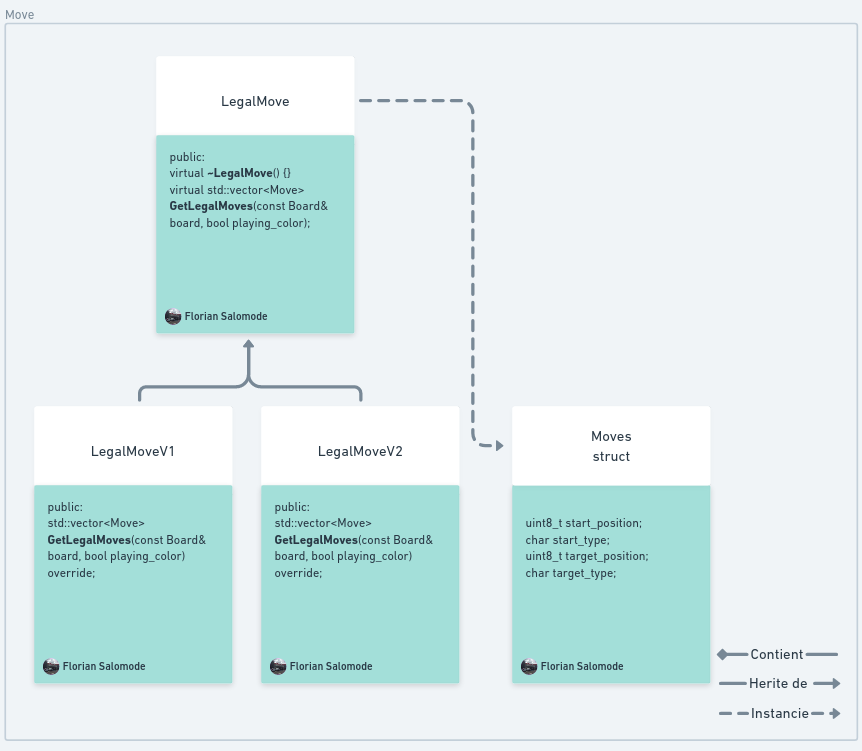
\includegraphics[scale = 0.3]{img/Package/Move.png}
    \caption{Paquetage Move de PDP CHESS}
    \label{pck:move}
\end{figure}
Le paquetage Move, quand à lui, gère tout ce qui est en rapport avec les mouvements des pièces, il contient la structure des mouvements, mais aussi les deux versions des mouvements légaux :
\begin{itemize}
    \item LegalMoveV1 [Voir \ref{mouvements_legaux_v1}]
    \item LegalMoveV2 [Voir \ref{mouvements_legaux_v2}]
\end{itemize}
Ils génèrent les listes de mouvements légaux possibles pour un joueur donné.
\medskip

Pour finir, le paquetage père, Engine, est "dirigé" par la classe Game qui articule la partie en contenant la boucle de jeu et un board dont elle appelle les différentes fonctions (Appliquer un mouvement \dots), jusqu'à l'arrêt de la partie.


\begin{figure}[!h]
    \centering
    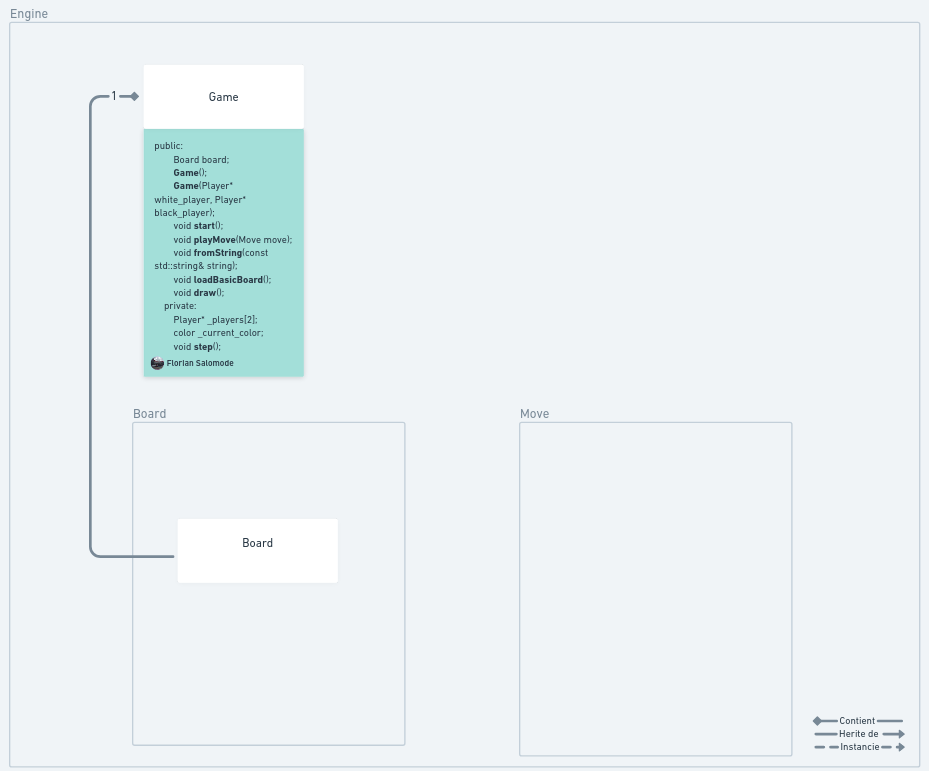
\includegraphics[scale = 0.3]{img/Package/Engine.png}
    \caption{Paquetage Engine de PDP CHESS}
    \label{pck:engine}
\end{figure}

\newpage
\paragraph{Valuation}
~~\\
\newline
Le paquetage de Valuation est tout simplement le paquetage contenant la fonction d'évaluation modulable [Voir \ref{heuristique_architecture}]
qui sera utilisée par les intelligences artificielles. [Voir \ref{player_architecture}]
\begin{figure}[!h]
    \centering
    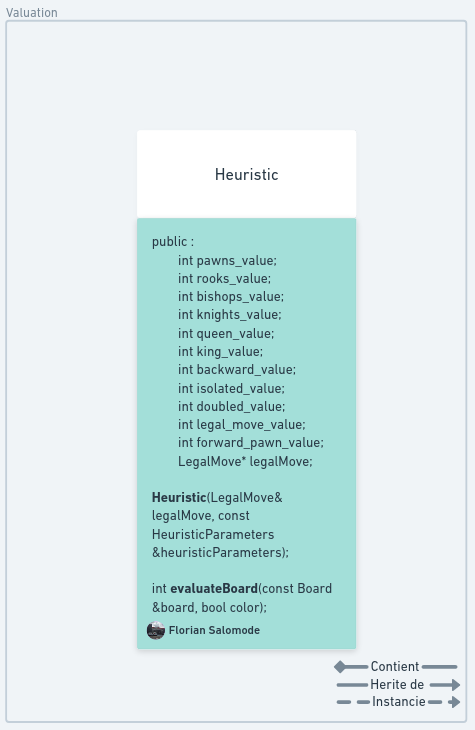
\includegraphics[scale = 0.2]{img/Package/Valuation.png}
    \caption{Paquetage Valuation de PDP CHESS}
    \label{pck:valuation}
\end{figure}


\paragraph{Player}
~~\\
\newline
Le paquetage Player contient tout ce qui est en rapport avec les joueurs.
Une PlayerFactory permet de générer n'importe quel type de joueur de manière automatisée suivant un fichier json [Voir \ref{json}].
Les types de joueurs sont redécoupés en 3 types distincts : 
\begin{itemize}
    \item Le RandomPlayer : joueur appliquant un mouvement aléatoire.
    \item Le HumanPlayer : l'utilisateur génère les mouvements.
    \item Les AIPlayer : sous-paquetage comprenant toutes les intelligences artificielles qui implémentent une interface AIPlayer.
    \newline
\end{itemize}

\begin{figure}[!h]
    \centering
    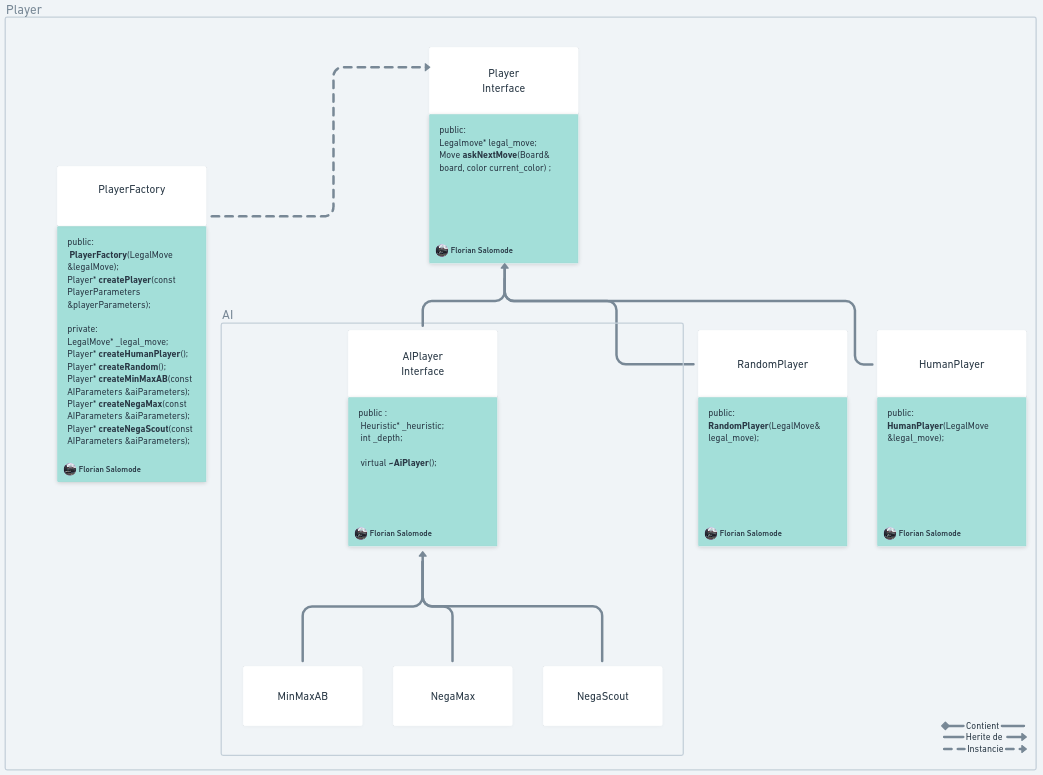
\includegraphics[scale = 0.40]{img/Package/Player.png}
    \caption{Paquetage Player et AI de PDP CHESS}
    \label{pck:player}
\end{figure}

\newpage
\paragraph{Util}
~~\\
\newline
Le paquetage Util est une boite à outils utilisée par plusieurs parties de l'application. Ce ne sont pas des classes mais un groupement de fonctions :
\begin{itemize}
    \item La fonction du vector\_shuffle est utilisée par les intelligences artificielle afin de randomiser les meilleurs coups, s'ils sont plusieurs.
    \item Le match\_parser est un groupe de fonctions permettant d'analyser une syntaxe et d'en retirer les informations attendues. Elles sont utilisées par le Director que nous verrons dans la section suivante [Voir \ref{pck:orchestration}] qui va l'utiliser pour passer d'un fichier json aux paramètres concrets d'initialisation d'une partie.
\end{itemize}
\begin{figure}[!h]
    \centering
    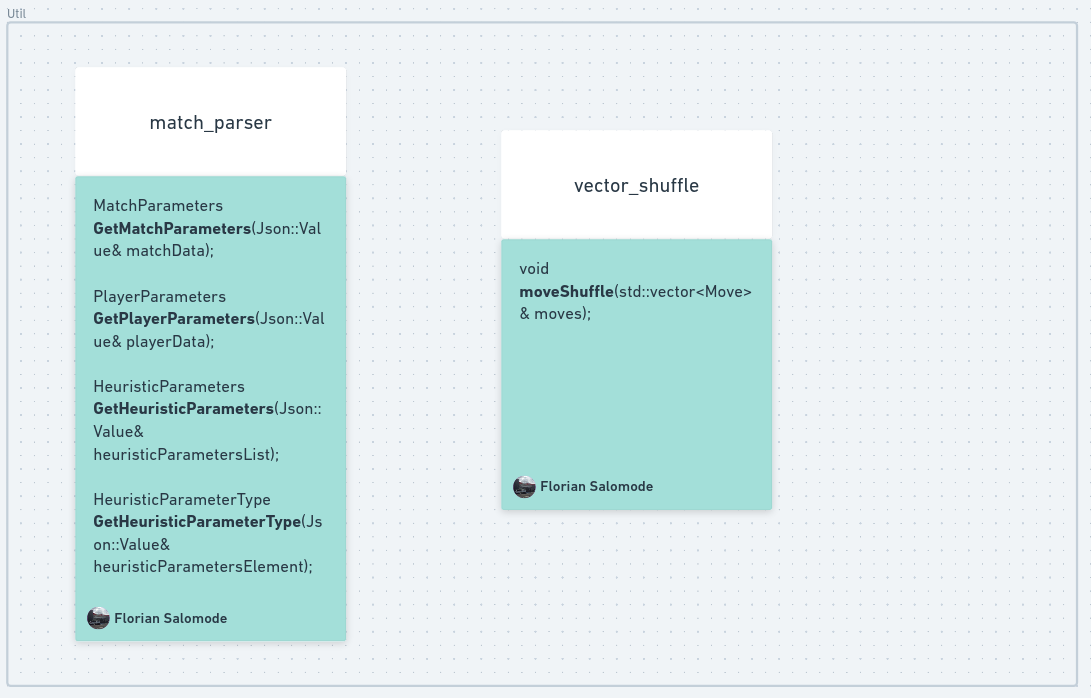
\includegraphics[scale = 0.3]{img/Package/Util.png}
    \caption{Paquetage Util de PDP CHESS}
    \label{pck:util}
\end{figure}
\newpage
\paragraph{Orchestration}
~~\\
\newline
Le paquetage Orchestration est constitué de la classe Director et d'un groupe de fonction parameters. Comme son nom l'indique, il a pour but d'orchestrer tous les préparatifs d'une partie en partant d'un fichier de configuration json, c'est à dire :
\begin{enumerate}
    \item Générer les bons types de joueurs, avec leurs bons paramètres ainsi que leur fonction d'évaluation de plateau (dans le cas d'une IA)
    \item Préparer un plateau de jeu classique ou personnalisé.
    \item Lancer la partie ou la réinitialiser au début.
\end{enumerate}

\begin{figure}[!h]
    \centering
    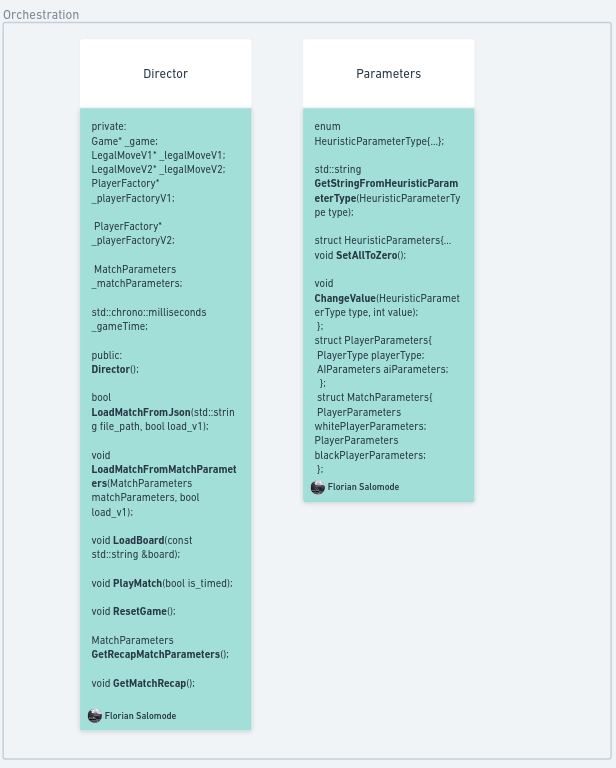
\includegraphics[scale = 0.3]{img/Package/Orchestration.png}
    \caption{Paquetage Orchestration de PDP CHESS}
    \label{pck:orchestration}
\end{figure}
\newpage
\subsubsection{Diagramme général}
~~\\
\newline
\begin{figure}[!h]
    \centering
    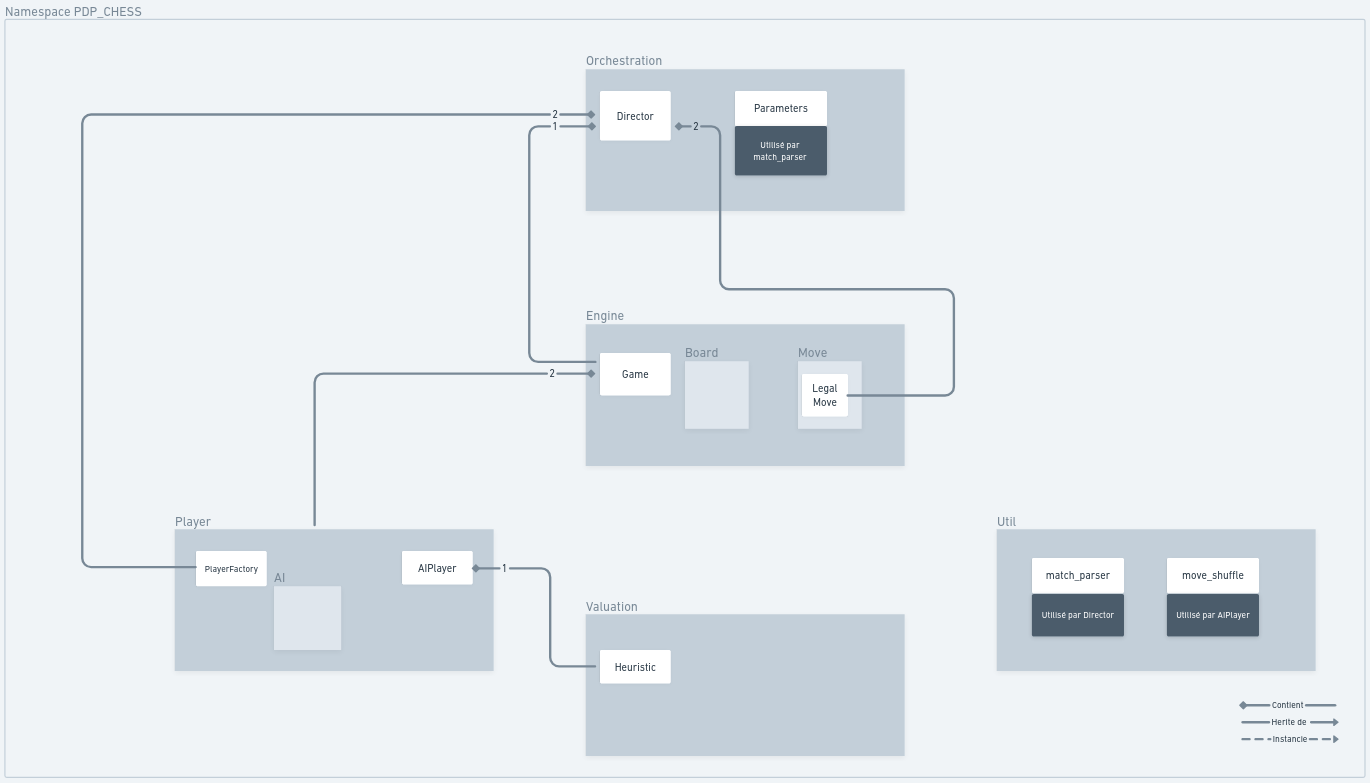
\includegraphics[scale = 0.35]{img/Package/UML.png}
    \caption{Diagramme UML de PDP CHESS}
    \label{uml}
\end{figure}
\newline 
Le programme entier est dans le même namespace (pdp\_chess).
Le diagramme UML ci-dessus du namespace pdp\_chess montre les connections entre les différents paquetages du programme.
Mettons nous dans une situation concrète d'un lancement de partie via un fichiers json, les différents liens entre les paquetages sont les suivants :
\begin{enumerate}
    \item le Director [Voir \ref{pck:orchestration}] via parameters et match\_parser instancie et contient une Game [Voir \ref{pck:engine}], deux LegalMove [Voir \ref{pck:move}], donc un pour chaque version des mouvements légaux, ainsi que deux PlayerFactory [Voir \ref{pck:player}] pour la même raison. Le tout à partir du fichier json passé en paramètre.
    \item Au moment de la création de Game, la classe Game crée et contient un Board [Voir \ref{pck:board}].
    \item Le Board, à sa création contient à son tour deux player\_state pour représenter les pions des 2 joueurs.
    \item le Director utilise la/les factory pour instancier les deux joueurs demandés avec leurs bons paramètres.
    \item Si les joueurs sont des AIPlayer, la factory instancie les Heuristics [Voir \ref{pck:valuation}] aux paramètres demandé et les fournit aux joueurs à leurs créations.
    \item Le Director place les 2 joueurs dans Game dans le respect de leurs couleurs.
    \item Le Director lance la partie. \dots
\end{enumerate}


\medskip

\newpage
\section{Tests}
\subsection{Tests unitaires}

\begin{itemize}
    \item \textbf{Legal move test :} \newline
    Dans ce fichier de test, nous avons un test pour chaque fonction qui renvoie des mouvements légaux, donc un pour les pions, un pour les tours etc\dots , ainsi qu'un test pour la fonction qui regroupe tout les mouvements possibles d'un joueur.\newline
    Le but de ces tests est de vérifier que les fonctions qui nous renvoient les mouvements possibles nous renvoient bien les bon mouvements.\newline
    Pour cela, nous allons utiliser des plateaux qui représentent des situations de jeu possibles, sachant que pour chaque cas (test sur les pions, test sur les tours...), nous avons un plateau spécifique à chacune des pièces à tester qui contient les situations les plus piégeuses, à la suite de ça, nous allons appeler la fonction que nous voulons tester sur ce plateau.\newline
    Pour vérifier le résultat qui en sort, nous nous assurons que tout les mouvements possibles qui en sortent sont bien des mouvements possibles attendus et qu'aucun ne manque sinon le test échouera.\newline
    
    \item \textbf{Condition isdraw test}\newline
    Dans ce fichier de test, nous testons si la fonction analyse bien le plateau et détecte le match nul quand il le faut.\newline
    Pour cela, nous avons des plateaux qui correspondent à chaque cas de match nul et nous vérifions que notre fonction nous renvoie bien que le match est nul sur ces plateaux.\newline
    Lorsque nous utilisons notre fonction sur un plateau considéré comme un match nul et qu'elle nous renvoie vraie et que lorsque nous l'utilisons sur un plateau considéré comme match non nul et qu'elle renvoie faux alors le test est validé sinon il ne l'est pas.\newline
    
    \item \textbf{Bitboard io test}\newline 
    Le but de cette suite de test est de vérifier qu'un plateau de jeu soit bien initialisé suivant les paramètres qu'on lui donne, et que les pièces soit bien disposées sur le plateau de jeu.\newline
    Il faut donc un plateau de jeu à initialiser : soit avec la méthode fromString qui, à partir d'une certaine chaîne de caractères construit le plateau qui en découle, soit via une méthode prédéfinis, comme la mise en place d'un plateau classique.\newline
    La comparaison du test se fera entre deux chaînes de caractères. 
    D'une part celle du plateau escompté donc ici, celle passée en paramètre au début, d'autre part, celle générée par le plateau de jeu via la fonction toString.
    Si les deux chaînes de caractères sont identiques, alors le test est déclaré valide.
    Dans les autres cas, il ne l'est pas.\newline
    
    
    \item \textbf{Bitboard move test} \newline
    L'objectif de ce fichier de test est de tester si un mouvement [Voir \ref{Mouvements}] appliqué sur un des bitboards \cite{Bitboards} des pièces est bien réalisé.\newline
    Pour ce faire, plusieurs plateaux de jeux sont prédéfinis, notamment pour les situations compliquées, ou à problèmes, par exemple lors d'une prise de pièce par une autre, ou il ne s'agit plus seulement de vérifier le bitboards de la pièce qui s'est déplacée, mais aussi celui de la pièce qui a été prise.\newline
    Nous effectuons donc le mouvement sur le plateau de jeu et nous comparons le ou les bitboards obtenus avec les bitboards escomptés.\newline
    S'ils sont égaux, alors le test est dit valide.
    Sinon, il n'est pas validé.\newline
    
    \item \textbf{bitboard operation test}\newline
    L'objectif de ce fichier est de tester si notre fonction "getPosition" nous renvoie les index des bits à 1 d'un bitboard passé en paramètres.\newline
    Pour cela, nous lançons notre fonction avec plusieurs bitboards différents et on compare les index qu'elle nous renvoie avec les index attendus.\newline
    Si l'ensemble des index attendus et l'ensemble des index donnés par notre fonction sont égaux alors le test est validé sinon il n'est pas validé.\newline
    
    \newpage
    \item \textbf{Heuristic test}\newline
    L'intention de cette suite de test est de vérifier que la fonction d'évaluation du plateau [Voir \ref{heuristique_contexte}]
    retourne la bonne valeur, et cela en se basant sur plusieurs critères : 
    \begin{itemize}
        \item le poids des pièces
        \item l'avancement des pions
        \item le nombre de mouvements légaux possible
    \end{itemize}
    Le test initialise donc un plateau de jeu prédéfini et lance la fonction d'évaluation du plateau sur celui-ci.\newline
    En parallèle, il stocke le résultat attendu afin de le comparer au résultat obtenu.\newline
    Si les résultats sont égaux alors le test est valide.
    S'ils sont différents, le test est déclaré non valide.
    
    
    
    
    
    
    
\end{itemize}
du test, et les moyens de mise en œuvre de cette analyse.
\subsection{Tests de performance}
\subsubsection{Moteur de jeu}
\paragraph{Protocole}
~~\\
\newline
Le contexte de ces tests est le suivant :
\begin{itemize}
    \item Le dossier de travail est un dossier de build dans /pdp\_echec/src/
    \item Test réalisé avec la commande "./version\_test 1" (1ère ligne)
    \item Test réalisé avec la commande "./version\_test 2" (2ème ligne)
    \item Commit du test (1ère colonne des résultats) : ec75eae2c3bed8b7c02709f877001576b541183d (SHA-1)
    \item Commit du test (2ème colonne des résultats) : 06198dc587a176543ddb48243e40a5bd5c8a12ed (SHA-1)
    \item Deux algorithmes AlphaBeta de profondeur 3 s'affrontent jusqu'à la fin de la partie.
    \item Pour obtenir une plus grande variété de plateaux, les algorithmes disposent d'une liste de mouvements légaux mélangée aléatoirement (seed dépendante de l'horloge interne).
    \item Le match n'est pas déterministe et est donc répété 200 fois pour obtenir la moyenne du temps d'exécution.
    \item L'heuristique possède ses paramètres par défaut.
    \item Le critère qui donne de l'importance au nombre de mouvements légaux disponible est utilisé, ce qui favorise la taille des mouvements légaux générés, et donc le nombre d'appels aux fonctions testées.
\end{itemize}


\paragraph{Résultats} \label{resultats_moteur}
~~\\
\newline
Ces résultats sont exprimés en millisecondes pour le temps moyen d'exécution.

\begin{center}
   \begin{tabular}{ | l | c | c | }
     \hline
      & Recherche exhaustive [\ref{recherche_bit_exhaustive}] & Recherche par soustraction [\ref{recherche_bit_soustraction}] \\ \hline
     Mouvements légaux V1 [\ref{mouvements_legaux_v1}] & 2006 & 1803 \\ \hline
     Mouvements légaux V2 [\ref{mouvements_legaux_v2}] & 3851 & 3442 \\
     \hline
   \end{tabular}
\end{center}

Nous prendrons donc les paramètres donnant le meilleur résultat pour tous les autres tests, c'est à dire la recherche par soustraction et les mouvements légaux V1.

\subsubsection{Algorithmes}
\paragraph{Protocole}
~~\\
\newline
Le contexte de ces tests est le suivant :
\begin{itemize}
    \item Le dossier de travail est un dossier de build dans /pdp\_echec/src/
    \item Commit des tests  : f3c88e4095c7286662bb440efa57160f9b271c92 (SHA-1)
    \item Tests réalisés avec les commandes : 
    \item "./speed\_test\_alphabeta x"
    \item "./speed\_test\_negamax x"
    \item "./speed\_test\_negascout x"
    \item x étant la profondeur voulue.
    \item Chaque algorithme (joueur blanc) à chaque profondeur se bat contre l'algorithme AlphaBeta de profondeur 1 avec heuristique classique jusqu'à la fin de la partie.
    \item L'affichage est désactivé
    \item Le match est déterministe et n'est donc pas répété.
    \item L'heuristique possède ses paramètres par défaut.
    \item Le critère qui donne de l'importance au nombre de mouvements légaux disponible est utilisé, ce qui favorise la taille des mouvements légaux générés, et donc le nombre d'appels aux fonctions testés.
\end{itemize}
\paragraph{Résultats}
~~\\
\newline
Ces résultats sont exprimés en millisecondes pour le temps d'exécution.
\begin{center}
   \begin{tabular}{ | l | c | c | c | }
     \hline
     Profondeur & AlphaBeta & NegaMax & Negascout \\ \hline
     1  & 3 & 3 & 3 \\ \hline
     2  & 17 & 55 & 22\\ \hline
     3  & 373 & 611 & 332\\ \hline
     4  & 3270 & 7623 & 2393\\ \hline
     5  & 115975 & 153144 & 38841\\ 
     \hline
   \end{tabular}
\end{center}

\section{Conclusion}

Nous avons atteint partiellement les objectifs de ce projet, en effet certaines règles du jeu ne sont pas implémentées tel que dans les règles officielles. Certains de nos algorithmes de recherche ne sont pas fonctionnels et l'algorithme NegaMax ne donne pas des résultats satisfaisants. \newline
De plus certains paramétrages ne sont pas disponibles après compilation notamment le gestion de l'aléatoire et du nombre de parties.
Finalement notre fichier de configuration n'est pas complètement résilient aux erreurs.\newline
Malgré ces problématiques non résolus, notre moteur de jeu possède plusieurs axes d'optimisation comparés. Nous avons implémenté différentes techniques de génération de mouvements parmi les techniques usuelles. \newline
Notre moteur de jeu est stable, les différents joueurs peuvent s'affronter dans des matchs paramétrables après compilation, et une grande partie des paramètres sont disponibles.

\section{Bibliographie}

\bibliographystyle{unsrt}
\bibliography{sample}

\end{document}